\chapter{Output Feedback and Offset-Free MPC}
\label{chap:output_fb_mpc}

\section{Introduction}
In the previous chapter, we derived Model Predictive Control under idealised assumptions: full state measurement, a perfect model, and no disturbances. Under these pure conditions, a simple regulator is sufficient to drive the system to the origin.

However, real-world control engineering is defined by its imperfections. Sensors are noisy and limited in number, meaning that the full state is rarely measurable. Models are merely approximations, failing to capture complex phenomena such as friction, aerodynamic drag or slowly varying biases. Furthermore, disturbances are rarely \emph{zero-mean}; a drone is subject to a constant gravitational force, and a building experiences continuous solar heat gains.

If we apply a standard MPC regulator to such a system, it will generally fail to track the reference exactly. The mismatch between the model's prediction and the plant's actual behaviour results in a permanent \emph{steady-state error} (or offset).

This chapter addresses these limitations. We introduce the \emph{output-feedback} framework, replacing the assumption of full-state access with a \emph{Kalman filter} that estimates the state from noisy measurements. We then develop \emph{offset-free MPC}~\cite{Pannocchia2003}: by augmenting the system model with a \textit{disturbance state} and employing a \textit{target calculator}, the MPC gains an integral-action-like capability. Under the usual observability, feasibility and modelling assumptions, this enables zero steady-state tracking error for constant or slowly varying disturbances and references.

\begin{notebox}{Connection to Classical Control}
	In PID control, steady-state error is eliminated by adding an \emph{integrator} term \(\frac{1}{s}\). In MPC, the same effect is achieved by \emph{estimating a disturbance} \(d\). In the language of the \textit{internal model principle}, augmenting the controller with a constant-disturbance model is closely related to embedding integral action.
\end{notebox}

\section{The Disturbance Model}

Standard LQR/MPC typically models plant uncertainty through zero-mean stochastic terms such as process noise \(w_k\). However, many practically important effects behave instead like persistent biases or slowly varying loads, such as gravity acting on a drone or solar gains acting on a building.

To handle this, we augment the system model with a \emph{disturbance state} \(d_k\), assumed constant or slowly varying:
\begin{align}
	x_{k+1} &= A x_k + B u_k + B_w d_k + w_k \label{eq:aug_sys_x}\\
	d_{k+1} &= d_k + \xi_k \label{eq:aug_sys_d}\\
	y_k &= C x_k + C_d d_k + v_k \label{eq:aug_sys_y}
\end{align}
where:
\begin{itemize}
	\item \(d_k \in \mathbb{R}^{n_d}\) is the integrating disturbance state.
	\item \(B_w\) determines how the disturbance enters the state equation. A common choice is the \emph{input-disturbance model}, in which \(B_w = B\), meaning that the disturbance acts through the same channel as the control input.
	\item \(C_d\) models disturbances that affect the output directly, for example a measurement bias.
	\item \(\xi_k\) is a \emph{fictitious} process-noise term. Physically, \(d_k\) may be constant, but we allow \(\xi_k\) in the estimator design so that the Kalman filter remains responsive if the real disturbance changes slowly over time.
\end{itemize}

\section{State and Disturbance Estimation}

Since the disturbance \(d_k\) is not ordinarily measurable, it must be estimated. The key idea is to treat the unknown disturbance as an additional state variable.

We therefore define the \emph{augmented state vector}
\[
z_k = \begin{bmatrix} x_k \\ d_k \end{bmatrix},
\]
and construct the corresponding augmented system:
\[
A_{\mathrm{aug}} =
\begin{bmatrix}
	A & B_w \\
	0 & I
\end{bmatrix}, \qquad
B_{\mathrm{aug}} =
\begin{bmatrix}
	B \\
	0
\end{bmatrix}, \qquad
C_{\mathrm{aug}} =
\begin{bmatrix}
	C & C_d
\end{bmatrix}.
\]

The identity matrix in the lower-right block of \(A_{\mathrm{aug}}\) expresses the modelling assumption that the disturbance remains constant from one step to the next unless the estimator sees evidence to the contrary.

A standard Kalman filter may now be designed for the augmented system \((A_{\mathrm{aug}}, C_{\mathrm{aug}})\). 

\begin{alertbox}{Observability Condition}
	For the disturbance to be estimable, the augmented pair \((A_{\mathrm{aug}}, C_{\mathrm{aug}})\) must be observable, or at least detectable. Intuitively, the available measurements must contain enough information to distinguish a change in the physical state \(x_k\) from a change in the disturbance \(d_k\).
	
	A useful practical rule of thumb is not to introduce more independent integrating-disturbance components than can be supported by the measured outputs. Otherwise, the augmented model is likely to become unobservable.
\end{alertbox}

\section{The Target Calculator}

To achieve offset-free tracking, we cannot simply drive the input towards zero. If a disturbance \(\hat d_k\) is pushing the system, the actuators must generally maintain a non-zero steady-state input \(u_{ss}\) in order to counteract it.

We therefore compute steady-state targets by solving the equilibrium equations. At steady state we require:
\begin{enumerate}
	\item The state to remain stationary,
	\[
	x_{ss} = A x_{ss} + B u_{ss} + B_w \hat d_k,
	\]
	\item The output to match the reference,
	\[
	r_k = C x_{ss} + C_d \hat d_k.
	\]
\end{enumerate}

\subsection{Method 1: Linear Solution (Unconstrained)}

In the simplest case, where the target is reachable and no steady-state constraints are enforced, the equations above reduce to the linear system
\begin{equation} \label{eq:target_calc}
	\begin{bmatrix}
		I - A & -B \\
		C & 0
	\end{bmatrix}
	\begin{bmatrix}
		x_{ss} \\
		u_{ss}
	\end{bmatrix}
	=
	\begin{bmatrix}
		B_w \hat d_k \\
		r_k - C_d \hat d_k
	\end{bmatrix}.
\end{equation}
If the coefficient matrix is nonsingular, this yields a computationally cheap steady-state target. However, it ignores actuator and state/output constraints, and therefore does not guarantee that the resulting target is physically reachable.

\subsection{Method 2: Constrained Optimisation (Robust)}

\begin{notebox}{The Reachability Problem}
	If the linear solution produces, for example, \(u_{ss} > u_{\max}\), then the target is infeasible. Feeding an unreachable target to the MPC regulator can compromise recursive feasibility and may lead to poor performance or failure.
\end{notebox}

To handle this, we reformulate the target calculation as a constrained \textbf{steady-state optimisation} (SSO) problem. Instead of insisting on exact equality \(y_{ss}=r_k\), we minimise the tracking error whilst enforcing the equilibrium equations and any relevant constraints.

At each time step, after estimating \(\hat d_k\), we solve
\begin{align}
	\min_{x_{ss},u_{ss}} \quad &
	\|C x_{ss} + C_d \hat d_k - r_k\|_Q^2 + \|u_{ss}\|_R^2
	\label{eq:target_qp}\\
	\text{subject to:} \quad &
	(I-A)x_{ss} - B u_{ss} = B_w \hat d_k, \nonumber\\
	&
	u_{\min} \le u_{ss} \le u_{\max}, \nonumber\\
	&
	x_{\min} \le x_{ss} \le x_{\max}, \nonumber
\end{align}
or, where more appropriate, output constraints may be imposed in place of state constraints.

\textbf{Advantages:}
\begin{itemize}
	\item The MPC is always asked to track a target that exists within the admissible set.
	\item If the reference \(r_k\) is unreachable, the SSO automatically returns the closest feasible operating point.
\end{itemize}

\section{The MPC Formulation}

\begin{figure}[htbp]
	\centering
	\begin{tikzpicture}[
		node distance = 1.8cm,
		auto,
		>=Latex,
		block/.style = {draw, rectangle, thick, minimum height=3em, minimum width=3.5em, align=center, fill=blue!5},
		plant/.style = {draw, rectangle, thick, minimum height=3em, minimum width=3.5em, fill=red!10, align=center},
		input/.style = {coordinate},
		output/.style = {coordinate}
		]
		
		\node [input] (input) {};
		\node [block, right=1cm of input, fill=purple!10] (target) {Target\\Calculator};
		\node [block, right=1.5cm of target, fill=blue!10] (mpc) {MPC\\Regulator};
		\node [plant, right=2.5cm of mpc] (plant) {Physical\\Plant};
		\node [output, right=1.5cm of plant] (output) {};
		
		\node [block, below=2.5cm of mpc, fill=cyan!10] (kf) {Augmented\\Observer};

		
		\draw [->, thick] (input) -- node[name=ref] {$r_k$} (target);
		\draw [->, thick] (target) -- node[above] {$x_{ss},\,u_{ss}$} (mpc);
		\draw [->, thick] (mpc) -- node[above, name=uk_node] {$u_k$} (plant);
		\draw [->, thick] (plant) -- node[name=y] (y_node) {$y_k$} (output);
		
		\node [above=0.8cm of plant] (dist) {Unknown disturbance \(d_k\)};
		\draw [->, thick, dashed] (dist) -- (plant);
		
		\draw [->, thick] (y_node.south) |- (kf.east);
		\fill (y_node.south) circle (1.5pt);
		\node at ($(mpc.south)!0.7!(plant.south) + (0, -2.8)$) {Measurement};
		
		\draw [->, thick] (kf.north) -- node[left, font=\small] {$\hat x_k$} ($(mpc.south) + (0., 0)$);
		\draw [->, thick] (kf.west) -| node[pos=0.25, above, font=\small] {$\hat{d}_k$}(target.south);
		
		\draw [->, thick] (uk_node.south) -- ++(0, -2.0) -| node[pos=0.85, above, font=\small] {$u_{k-1}$} ($(kf.north) + (0.6, 0)$);
		\fill (uk_node.south) circle (1.5pt);
		
		\node [draw=gray, dashed, inner sep=10pt, fit=(kf), label=below:\small\textit{Observer Block}] (obs_box) {};
		
	\end{tikzpicture}
	\caption{Offset-free control architecture. The target calculator uses the  disturbance estimate \(\hat d_k\) to compute the steady-state targets \((x_{ss},u_{ss})\). The MPC regulator steers the system towards these targets using the estimated state \(\hat x_k\). The augmented observer uses the measurement \(y_k\) and the previously applied control input \(u_{k-1}\). The disturbance filter is optional and is included here to reduce noise in the disturbance estimate.}
	\label{fig:offset_free_architecture}
\end{figure}

\begin{notebox}{Separation principle caveat}
The certainty-equivalence approach --- using the Kalman filter estimate $\hat{x}_k$ as if it were the true state --- is exact for unconstrained LQG. For constrained MPC, this separation no longer holds rigorously: the estimator and controller interact through the constraints. In practice, the combined observer--MPC architecture works well, but formal closed-loop guarantees require additional analysis (e.g.\ inherent robustness of MPC or robust output-feedback MPC formulations).
\end{notebox}

\begin{figure}[htbp]
	\centering
	\resizebox{\textwidth}{!}{
\begin{tikzpicture}[
	auto, >=Latex, node distance = 2.5cm,
	block/.style  = {draw, rectangle, thick, minimum height=3.3cm, minimum width=4.8cm,
		align=center, fill=blue!5, rounded corners=2pt, font=\footnotesize},
	plant/.style  = {draw, rectangle, thick, minimum height=3.3cm, minimum width=4.8cm,
		fill=red!10, align=center, font=\footnotesize},
	filter/.style = {draw, rectangle, thick, minimum height=3.0cm, minimum width=3.8cm,
		align=center, fill=cyan!10, rounded corners=2pt, font=\footnotesize},
	input/.style  = {coordinate},
	output/.style = {coordinate}
	]
	
	\node [input] (input) {};
	
	\node [block, right=1.2cm of input, fill=blue!10] (target) {
		\textbf{Target Calculator}\\[0.4em]
		Simple tracking case:\\[0.2em]
		\(
		\begin{bmatrix} I\!-\!A & -B\\ C & 0 \end{bmatrix}
		\begin{bmatrix} x_{ss}\\ u_{ss} \end{bmatrix}
		=
		\begin{bmatrix} B_w \hat d_k\\ r_k - C_d \hat d_k \end{bmatrix}
		\)\\[0.4em]
		or solve a constrained steady-state optimisation
	};
	
	\node [block, right=1.5cm of target, fill=blue!10] (mpc) {
		\textbf{MPC Regulator}\\[0.4em]
		\(
		\min \displaystyle\sum_{i=0}^{N-1}
		\bigl(\|\tilde x_i\|_Q^2 + \|\tilde u_i\|_R^2 + \rho\|\epsilon_i\|^2\bigr)
		+ \|\tilde x_N\|_P^2
		\)\\[0.4em]
		subject to\\
		\(\tilde x_0 = \hat x_k - x_{ss}\)\\
		\(\tilde x_{i+1} = A\tilde x_i + B\tilde u_i\)\\
		\(u_{\min} \le \tilde u_i + u_{ss} \le u_{\max}\)\\
		\(y_{\min,i}-\epsilon_i \le C(\tilde x_i+x_{ss}) \le y_{\max,i}+\epsilon_i\)\\
		\(\epsilon_i \ge 0\)
	};
	
	\node [plant, right=2.0cm of mpc] (plant) {
		\textbf{Physical Plant}\\[0.5em]
		\(x_{k+1} = A x_k + B u_k + B_w d_k + w_k\)\\[0.3em]
		\(y_k = C x_k + C_d d_k + v_k\)
	};
	
	\node [output, right=1.5cm of plant] (output) {};
	
	\node [filter, below=3cm of mpc, xshift=0cm] (kf) {
		\textbf{Augmented Observer}\\[0.4em]
		\(\hat z_{k|k-1} = A_{\mathrm{aug}}\hat z_{k-1|k-1} + B_{\mathrm{aug}}u_{k-1}\)\\[0.3em]
		\(\hat z_{k|k} = \hat z_{k|k-1} + L\!\left(y_k - C_{\mathrm{aug}}\hat z_{k|k-1}\right)\)\\[0.4em]
		{\scriptsize State: \(\hat z_k = [\hat x_k^\top,\ \hat d_k^\top]^\top\)}  % 
	};
	
	%% ── Forward path ─────────────────────────────────────────────
	\draw [->, thick] (input) -- node[name=ref] {$r_k$} (target);
	\draw [->, thick] (target) -- node[above] {$x_{ss},\,u_{ss}$} (mpc);
	\draw [->, thick] (mpc) -- node[above, name=uk_line] {$u_k$} (plant);
	\draw [->, thick] (plant) -- node[name=y] (y_node) {$y_k$} (output);
	
	\node [above=0.8cm of plant] (dist) {Unknown \(d_k\)};
	\draw [->, thick, dashed] (dist) -- (plant);
	
	%% ── Feedback paths ───────────────────────────────────────────
	\draw [->, thick] (y_node.south) |- (kf.east);
	\fill (y_node.south) circle (2pt);
	\node at ($(plant.south) + (1.0,-1.5)$) {Measurement};
	
	\draw [->, thick] (kf) -| node[left] {$\hat d_{k}$} (target);
	\draw [->, thick] (kf.north) -- ++(0,0.5)
	-| node[pos=0.05, above] {$\hat x_k$} ($(mpc.south) + (0.5,0)$);
	
	\draw [->, thick] (uk_line.south) -- ++(0,-2.5)
	-| node[pos=0.8, above] {$u_{k-1}$} ($(kf.north) + (1.75,0)$);
	\fill (uk_line.south) circle (2pt);
	
	%% ── Observer bounding box ────────────────────────────────────
	\node [draw=gray, dashed, inner sep=10pt, fit=(kf),          % ← FIX: restored full \node
	label=below:\small\textit{Observer Block}] (obs_box) {};
	
\end{tikzpicture}

	}
	\caption{Detailed offset-free control architecture. The target calculator may be implemented either as the simple linear equilibrium solve of \eqref{eq:target_calc} or, more generally, as a constrained steady-state optimisation. The regulator is shown with soft output constraints, matching the examples developed later in the chapter.}
	\label{fig:offset_free_architecture_detailed}
\end{figure}

The complete control architecture is illustrated in Figure~\ref{fig:offset_free_architecture}, with detailed mathematical definitions shown in Figure~\ref{fig:offset_free_architecture_detailed}.

\subsection{Control Topology}

The architecture operates as a hierarchical loop, separating the task of \emph{setpoint determination} from the task of \emph{regulation}. The information flow at time step \(k\) is as follows:

\begin{enumerate}
	\item \textbf{Observer Block:} The cycle begins with the measurement \(y_k\). The \emph{augmented observer} fuses this measurement with the previously applied input \(u_{k-1}\) to produce an estimate of the physical state \(\hat x_k\) and the raw disturbance estimate \(\hat d_{\mathrm{raw},k}\). To prevent high-frequency sensor noise from propagating into the controller, the disturbance estimate may be smoothed by a \emph{disturbance filter}, yielding \(\hat d_k\).
	
	\item \textbf{Target Calculator:} This block acts as the bridge between the external reference and the controller. It takes the reference \(r_k\) and the estimated disturbance \(\hat d_k\) as inputs. By solving the equilibrium equations, or more generally a constrained steady-state optimisation problem, it computes the target state \(x_{ss}\) and target input \(u_{ss}\). These represent an operating point at which the output matches the reference whilst compensating for the estimated disturbance.
	
	\item \textbf{MPC Regulator:} Finally, the MPC regulator receives the current state estimate \(\hat x_k\) together with the calculated targets \((x_{ss},u_{ss})\). Its role is to steer the system from \(\hat x_k\) towards \(x_{ss}\) whilst satisfying the imposed constraints.
\end{enumerate}

\subsection{Optimisation Problem}

Once the steady-state targets \((x_{ss}, u_{ss})\) have been computed, the
regulation layer is designed in \textbf{deviation variables}:
\[
\tilde x_i = x_i - x_{ss}, \qquad \tilde u_i = u_i - u_{ss}.
\]
The full plant prediction model at step $i$ inside the horizon follows
from~\eqref{eq:aug_sys_x} with noise terms set to zero (certainty
equivalence) and the disturbance replaced by its current estimate
$\hat d_k$:
\[
x_{i+1} = A x_i + B u_i + B_w \hat d_k.
\]
The steady-state pair $(x_{ss}, u_{ss})$ satisfies the equilibrium
condition obtained by setting $x_{k+1} = x_k = x_{ss}$ and
$d_k = \hat d_k$ in~\eqref{eq:aug_sys_x}--\eqref{eq:aug_sys_d}:
\[
x_{ss} = A x_{ss} + B u_{ss} + B_w \hat d_k,
\qquad
y_{ss} = C x_{ss} + C_d \hat d_k.
\]
Subtracting the equilibrium equation from the prediction model gives
\begin{align*}
	x_{i+1} - x_{ss}
	&= A(x_i - x_{ss}) + B(u_i - u_{ss})
	+ \underbrace{B_w \hat d_k - B_w \hat d_k}_{=\;0}.
\end{align*}
Because the steady-state pair absorbs the disturbance estimate $\hat d_k$
through both the state equation and the output equation, all affine terms
cancel exactly, leaving the \textbf{disturbance-free linear deviation
	dynamics}:
\[
\tilde x_{i+1} = A \tilde x_i + B \tilde u_i.
\]
\begin{notebox}{Notation: Real Time vs Prediction Horizon}
	MPC operates on two distinct time scales:
	\begin{itemize}
		\item \(k\) denotes the current \emph{real-time} sampling instant.
		\item \(i\) denotes the \emph{prediction step} within the horizon.
	\end{itemize}
	Thus, \(\hat x_k\) is the current estimated state, whereas \(\tilde x_i\) is the predicted deviation \(i\) steps ahead within the optimisation.
\end{notebox}

A standard offset-free tracking MPC problem is
\begin{align}
	\min_{\tilde u_0,\ldots,\tilde u_{N-1},\,\epsilon_0,\ldots,\epsilon_{N-1}} \quad &
	\sum_{i=0}^{N-1}
	\left(
	\|\tilde x_i\|_Q^2 + \|\tilde u_i\|_R^2 + \rho\|\epsilon_i\|^2
	\right)
	+ \|\tilde x_N\|_{P_{\mathrm{term}}}^2
	\label{eq:mpc_problem}\\
	\text{subject to:} \quad &
	\tilde x_0 = \hat x_k - x_{ss}, \nonumber\\
	&
	\tilde x_{i+1} = A\tilde x_i + B\tilde u_i, \qquad i=0,\ldots,N-1, \nonumber\\
	&
	u_{\min} \le \tilde u_i + u_{ss} \le u_{\max}, \nonumber\\
	&
	y_{\min,i} - \epsilon_i
	\le
	C(\tilde x_i + x_{ss})
	\le
	y_{\max,i} + \epsilon_i, \nonumber\\
	&
	\epsilon_i \ge 0, \qquad i=0,\ldots,N-1. \nonumber
\end{align}
If \(C_d \neq 0\), the corresponding term \(C_d \hat d_k\) should also be included in the predicted output equation. In the examples below, \(C_d=0\), so the simpler form above is sufficient.

\begin{notebox}{Topology Insight}
	The initialisation constraint
	\[
	\tilde x_0 = \hat x_k - x_{ss}
	\]
	is the key link between the \emph{observer} and the \emph{target calculator}. The observer supplies \(\hat x_k\), the target calculator supplies \(x_{ss}\), and the MPC regulator penalises deviations from this target.
	
	Because the cost function penalises \(\tilde x_i\) and \(\tilde u_i\) rather than the absolute input \(u_i\), the controller is not penalised for maintaining the non-zero steady-state input \(u_{ss}\) required to reject the disturbance.
\end{notebox}

The control input applied to the plant is
\[
u_k = \tilde u_0^\star + u_{ss},
\]
possibly followed by a final saturation step for numerical safety.

\subsection{Handling Infeasibility: Hard vs Soft Constraints}

In an ideal world, the MPC solver always finds a trajectory satisfying every constraint. In reality, disturbances, model mismatch or estimation errors may push the system into a region from which it is impossible to satisfy all limits simultaneously. If the feasible set becomes empty, the optimisation problem fails.

To improve robustness, it is useful to distinguish between two types of constraints.

\subsubsection*{Hard Constraints (Inputs)}
Input constraints represent immutable physical limits of the actuators, such as the maximum voltage of a motor or the fully open position of a valve. Since the controller cannot command an actuator beyond its physical capability, input constraints should normally be modelled as \emph{hard constraints}.

\subsubsection*{Soft Constraints (States/Outputs)}
State or output constraints often represent safety or performance requirements. If a large disturbance makes one of these temporarily impossible to satisfy, a hard constraint would render the optimisation infeasible exactly when corrective action is most needed. To avoid this, such constraints are often softened by introducing a slack variable.

\subsubsection*{Mathematical Implementation}
We introduce a non-negative \emph{slack variable} \(\epsilon_i \ge 0\), which acts as a safety valve for the soft constraints. Ideally, \(\epsilon_i=0\). To encourage this, we add a large penalty weight \(\rho\) to the cost function. The modified problem is
\begin{align*}
	\min_{\tilde u,\epsilon} \quad &
	\sum_{i=0}^{N-1}
	\left(
	\|\tilde x_i\|_Q^2 + \|\tilde u_i\|_R^2 + \rho\|\epsilon_i\|^2
	\right)
	+ \|\tilde x_N\|_{P_{\mathrm{term}}}^2 \\
	\text{subject to:} \quad &
	\tilde x_{i+1} = A\tilde x_i + B\tilde u_i, \\
	&
	u_{\min} \le \tilde u_i + u_{ss} \le u_{\max}, \\
	&
	y_{\min,i} - \epsilon_i
	\le
	C(\tilde x_i + x_{ss})
	\le
	y_{\max,i} + \epsilon_i, \\
	&
	\epsilon_i \ge 0.
\end{align*}

\begin{notebox}{Interpretation}
	Because \(\rho\) is chosen to be very large, the optimiser keeps \(\epsilon_i = 0\) whenever possible, so that the soft constraint behaves like a hard one. If, however, the strict bound is temporarily impossible to satisfy, the optimiser increases \(\epsilon_i\) only as much as necessary to maintain feasibility.
\end{notebox}

\begin{examplebox}{MATLAB: Offset-Free MPC with Disturbance Estimation}
	
	\textbf{Problem Formulation:}\\
	
	We consider a second-order discrete-time linear system subject to measurement noise and an unknown piecewise-constant input disturbance. The objective is to track a piecewise-constant reference \(r_k\) whilst respecting hard input constraints and soft output constraints.
	
	\textbf{System Dynamics:}\\
	
	\begin{align*}
		x_{k+1} &= A x_k + B u_k + B_w d_k \\
		y_k &= C x_k + v_k
	\end{align*}
	where the system matrices are
	\[
	A = \begin{bmatrix} 0.9535 & 0.0761 \\ -0.8454 & 0.5478 \end{bmatrix}, \quad
	B = \begin{bmatrix} 0.0465 \\ 0.8454 \end{bmatrix}, \quad
	B_w = B, \quad
	C = \begin{bmatrix} 1 & 0 \end{bmatrix}.
	\]
	
	\textbf{Constraints:}
	\begin{itemize}
		\item Hard input saturation: \(-5 \le u_k \le 5\),
		\item Soft output bounds: \(-0.5 \le y_k \le 0.5\).
	\end{itemize}
	
	\textbf{Solution Strategy:}\\
	
	A standard MPC controller based on the nominal model would exhibit a steady-state offset in the presence of the unknown disturbance. The offset-free implementation therefore uses three components:
	
	\begin{enumerate}
		\item \textbf{Augmented Kalman Filter:} The state is augmented with a constant disturbance model,
		\[
		z_k =
		\begin{bmatrix}
			x_k\\
			d_k
		\end{bmatrix}, \qquad
		z_{k+1} =
		\begin{bmatrix}
			A & B_w\\
			0 & 1
		\end{bmatrix} z_k +
		\begin{bmatrix}
			B\\
			0
		\end{bmatrix} u_k,
		\]
		and a Kalman filter provides estimates \(\hat x_k\) and \(\hat d_k\).
		
		\item \textbf{Target Calculator:} The estimated disturbance is used to compute the steady-state operating point \((x_{ss},u_{ss})\) satisfying
		\[
		(I-A)x_{ss} - B u_{ss} = B_w \hat d_k,
		\qquad
		Cx_{ss} = r_k.
		\]
		
		\item \textbf{Deviation-Form MPC:} The regulator then solves an MPC problem in deviation coordinates \(\tilde x_i = x_i - x_{ss}\), \(\tilde u_i = u_i - u_{ss}\), with soft output constraints and hard input constraints.
	\end{enumerate}
	
	\textbf{MATLAB Implementation:}\\
	
	\begin{lstlisting}[language=Matlab]
	clear; clc; close all; rng(1);
	
	%% 1. System Definition
	A  = [0.9535  0.0761; -0.8454  0.5478];
	B  = [0.0465 ; 0.8454];
	Bw = B;
	C  = [1 0];
	
	nx = 2; nu = 1; ny = 1;
	
	u_min = -5;  u_max =  5;
	y_min = -0.5; y_max =  0.5;
	
	%% 2. Augmented Observer
	% Augmented state: z_k = [x_k; d_k],  d_{k+1} = d_k
	A_aug = [A, Bw; zeros(1,nx), 1];
	B_aug = [B; 0];
	C_aug = [C, 0];
	
	% W(3,3) is the single tuning knob for disturbance tracking bandwidth
	W = diag([1e-4, 1e-4, 1e-4]);   % Kalman filter tuning weights
	V = 1e-3;                        % Measurement noise variance
	
	[P_ss, ~, ~] = dare(A_aug', C_aug', W, V);
	L = P_ss * C_aug' / (C_aug * P_ss * C_aug' + V);
	
	%% 3. Target Calculator
	% [I-A  -B] [x_ss]   [Bw * d_hat]
	% [ C    0] [u_ss] = [   ref    ]
	M_target = [eye(nx)-A, -B; C, zeros(ny,nu)];
	
	if rank(M_target) < (nx + nu)
		error('Target calculator matrix is rank deficient.');
	end
	
	%% 4. MPC Formulation
	N   = 20;
	q_y = 10;
	R   = 0.1;
	rho = 1e5;
	
	Q_state = C' * q_y * C;
	[P_N, ~, ~] = dare(A, B, Q_state, R);
	
	du    = sdpvar(nu, N,   'full');
	dx    = sdpvar(nx, N+1, 'full');
	slack = sdpvar(ny, N,   'full');
	
	x_hat = sdpvar(nx, 1);
	x_ss  = sdpvar(nx, 1);
	u_ss  = sdpvar(nu, 1);
	
	obj  = 0;
	cons = [dx(:,1) == x_hat - x_ss];
	
	for k = 1:N
		cons = [cons, dx(:,k+1) == A*dx(:,k) + B*du(:,k)];
		
		dy_k = C * dx(:,k);
		obj  = obj + dy_k'*q_y*dy_k + du(:,k)'*R*du(:,k) + rho*slack(:,k)'*slack(:,k);
		
		u_abs = du(:,k) + u_ss;
		y_abs = C * (dx(:,k) + x_ss);
		
		cons = [cons, u_min <= u_abs <= u_max];
		cons = [cons, y_min - slack(:,k) <= y_abs <= y_max + slack(:,k)];
		cons = [cons, slack(:,k) >= 0];
	end
	
	obj = obj + dx(:,N+1)' * P_N * dx(:,N+1);
	
	ops = sdpsettings('solver', 'quadprog', 'verbose', 0);
	mpc_controller = optimizer(cons, obj, ops, {x_hat, x_ss, u_ss}, {du(:,1), slack(:,1)});
	
	%% 5. Simulation Setup
	T_sim = 300;
	x_true = zeros(nx, 1);
	z_hat  = zeros(nx+1, 1);
	u_applied = 0;
	
	ref_signal = [repmat( 0.4,1,100), repmat(-0.4,1,100), repmat( 0.4,1,100)];
	w_true     = [repmat( 0.2,1,150), repmat(-0.2,1,150)];
	
	log_y_true = zeros(1,T_sim);  log_y_meas = zeros(1,T_sim);
	log_ref    = zeros(1,T_sim);  log_u      = zeros(1,T_sim);
	log_u_ss   = zeros(1,T_sim);  log_d_true = zeros(1,T_sim);
	log_d_hat  = zeros(1,T_sim);  log_slack  = zeros(1,T_sim);
	log_x1     = zeros(1,T_sim);  log_x2     = zeros(1,T_sim);
	
	fprintf('Starting simulation...\n');
	
	%% 6. Simulation Loop
	for t = 1:T_sim
	
		ref = ref_signal(t);
		
		% A. Plant output
		y_true = C * x_true;
		y_meas = y_true + sqrt(V) * randn;
		
		% B. Observer
		z_hat_pred = A_aug * z_hat + B_aug * u_applied;
		z_hat      = z_hat_pred + L * (y_meas - C_aug * z_hat_pred);
		
		x_hat_k = z_hat(1:nx);
		d_hat_k = z_hat(nx+1);
		
		% C. Target calculator
		targets = M_target \ [Bw * d_hat_k; ref];
		x_ss_k  = targets(1:nx);
		u_ss_k  = targets(nx+1:end);
		
		% D. MPC
		[sol, diagnostics] = mpc_controller{x_hat_k, x_ss_k, u_ss_k};
		
		if diagnostics == 0
			du_opt    = full(sol{1});
			slack_now = full(sol{2});
		else
			warning('MPC infeasible at t = %d (code %d). Applying u_ss.', t, diagnostics);
			du_opt    = 0;
			slack_now = NaN;
		end
		
		u_applied = min(max(du_opt + u_ss_k, u_min), u_max);
		
		% E. Plant update
		x_true = A * x_true + B * u_applied + Bw * w_true(t);
		
		% F. Logging
		log_y_true(t) = y_true;  log_y_meas(t) = y_meas;
		log_ref(t)    = ref;     log_u(t)      = u_applied;
		log_u_ss(t)   = u_ss_k;  log_d_true(t) = w_true(t);
		log_d_hat(t)  = d_hat_k; log_slack(t)  = slack_now;
		log_x1(t)     = x_true(1); log_x2(t)   = x_true(2);
	end

	
	%% Visualisation omitted for brevity.
	
	\end{lstlisting}
	Figure~\ref{fig:offset_free_results} shows the closed-loop output, the control signals, the disturbance estimate and the activity of the soft output constraint.
\end{examplebox}

\begin{figure}[!htb]
	\centering
	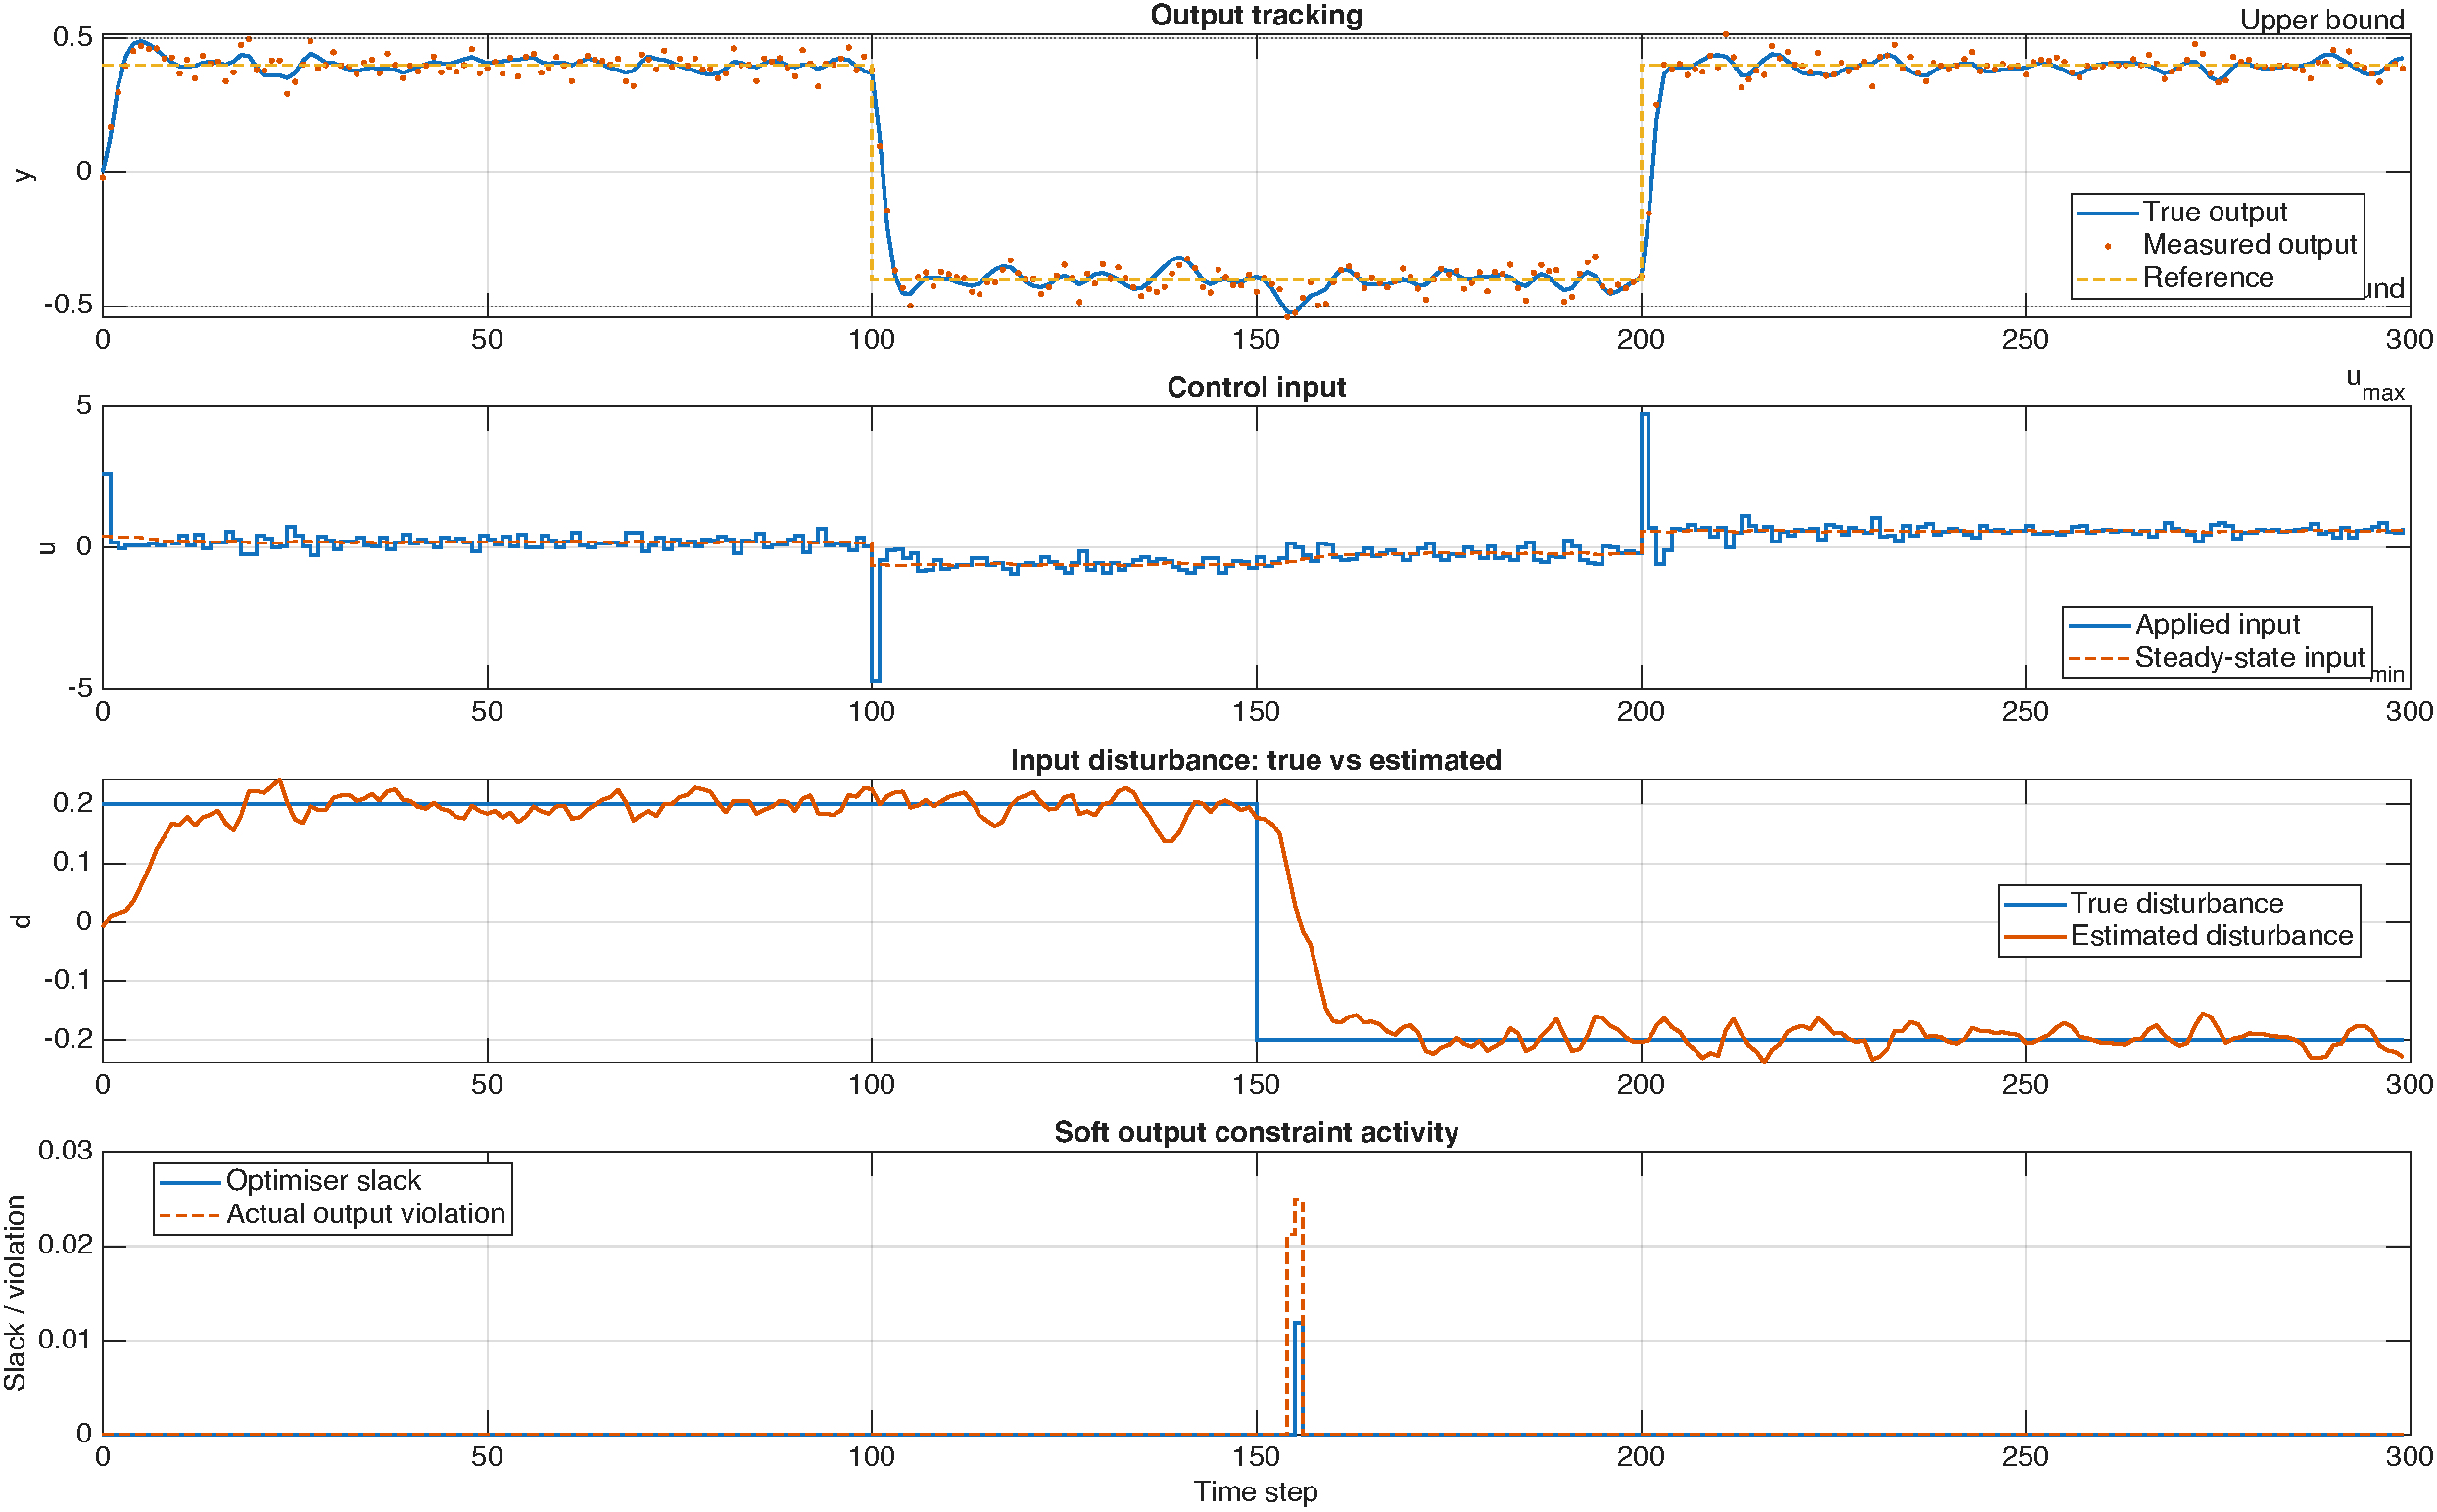
\includegraphics[width=1.0\linewidth]{Figures/Offsetfree_MPC.pdf}
	\caption{Closed-loop performance of the offset-free MPC with soft output constraints under piecewise-constant reference changes and an unknown step disturbance. The top panel shows accurate output tracking of the constrained reference whilst keeping the output close to the prescribed bounds. The second panel shows the applied control input together with the steady-state target input, with brief transient peaks at the reference-switching instants. The third panel shows that the augmented observer estimates the constant input disturbance well, including the disturbance sign change. The bottom panel shows that the soft output constraint is active only briefly during the disturbance transition, indicating that constraint violations are small and short-lived.}
	\label{fig:offset_free_results}
\end{figure}

The code follows the algorithm summarised in Algorithm~\ref{alg:offset_free_mpc}.

\begin{algorithm}
	\caption{Offset-Free MPC with Disturbance Estimation}
	\label{alg:offset_free_mpc}
	\begin{algorithmic}[1]
		\State \textbf{Input:} System matrices \((A,B,B_w,C)\), optional output-bias matrix \(C_d\), weights \((Q,R,P_{\mathrm{term}},\rho)\), input/output constraints, prediction horizon \(N\).
		\State \textbf{Output:} Control input \(u_k\).
		
		\Procedure{Offline Initialisation}{}
		\State Construct the augmented model
		\[
		z_k=
		\begin{bmatrix}
			x_k\\
			d_k
		\end{bmatrix},\qquad
		z_{k+1}=A_{\mathrm{aug}}z_k+B_{\mathrm{aug}}u_k,\qquad
		y_k=C_{\mathrm{aug}}z_k .
		\]
		\State Compute the estimator gain \(L\) from the DARE associated with \((A_{\mathrm{aug}},C_{\mathrm{aug}},W,V)\).
		\State Compute the terminal cost matrix \(P_{\mathrm{term}}\) for the deviation dynamics.
		\State Define the parametric MPC problem:
		\begin{align*}
			\min_{\tilde u,\epsilon}\quad
			&\sum_{i=0}^{N-1}
			\left(
			\|\tilde x_i\|_Q^2+\|\tilde u_i\|_R^2+\rho\|\epsilon_i\|^2
			\right)
			+\|\tilde x_N\|_{P_{\mathrm{term}}}^2 \\
			\text{s.t.}\quad
			&\tilde x_0=\hat x_k-x_{ss},\\
			&\tilde x_{i+1}=A\tilde x_i+B\tilde u_i,\qquad i=0,\dots,N-1,\\
			&u_{\min}\le \tilde u_i+u_{ss}\le u_{\max},\\
			&y_{\min,i}-\epsilon_i\le C(\tilde x_i+x_{ss})\le y_{\max,i}+\epsilon_i,\\
			&\epsilon_i\ge 0,\qquad i=0,\dots,N-1.
		\end{align*}
		\State Compile the solver object, including any real-time parameters required by the chosen formulation.
		\EndProcedure
		
		\Procedure{Online Control Loop}{}
		\State Initialise \(\hat z_{0|0}\), \(u_{-1}\), and optionally \(\hat d_{0}\).
		\For{$k=0,1,2,\dots$}
		\State Measure the output \(y_k\).
		
		\State \textit{// 1. Augmented-state estimation}
		\State \(\hat z_{k|k-1}\gets A_{\mathrm{aug}}\hat z_{k-1|k-1}+B_{\mathrm{aug}}u_{k-1}\)
		\State \(\hat z_{k|k}\gets \hat z_{k|k-1}+L\bigl(y_k-C_{\mathrm{aug}}\hat z_{k|k-1}\bigr)\)
		\State Extract \(\hat x_k\) and the raw disturbance estimate \(\hat d_{,k}\) from \(\hat z_{k|k}\).
	
		
		\State \textit{// 2. Steady-state target calculation}
		\State Compute \((x_{ss},u_{ss})\) from the current reference and disturbance estimate, either
		\[
		x_{ss}=Ax_{ss}+Bu_{ss}+B_w\hat d_k,\qquad
		r_k=Cx_{ss}+C_d\hat d_k,
		\]
		or, more generally, by solving a constrained steady-state optimisation problem.
		
		\State \textit{// 3. MPC regulation}
		\State Solve the MPC problem using the current parameters \((\hat x_k,x_{ss},u_{ss})\) and any future bound sequences if required.
		\State Obtain the first optimal move \(\tilde u_0^\star\).
		
		\State \textit{// 4. Apply input}
		\State \(u_k \gets \tilde u_0^\star + u_{ss}\)
		\State \(u_k \gets \max(u_{\min},\min(u_{\max},u_k))\)
		\State Apply \(u_k\) to the plant.
		\EndFor
		\EndProcedure
	\end{algorithmic}
\end{algorithm}

\noindent\textbf{Note.}
Algorithm~\ref{alg:offset_free_mpc} describes the general offset-free MPC structure based on augmented-state disturbance estimation, steady-state target calculation and deviation-form regulation. In the simplest reference-tracking case, the steady-state pair \((x_{ss},u_{ss})\) may be obtained directly from the linear equilibrium equations \eqref{eq:target_calc}. In constrained or economic MPC, however, it is generally more appropriate to compute \((x_{ss},u_{ss})\) by solving a constrained steady-state optimisation problem. Moreover, if soft output constraints are used, the slack variables must satisfy \(\epsilon_i \ge 0\), and the indexing of predicted outputs in the constraints should be chosen consistently with the state-update convention adopted in the MPC formulation.

\begin{examplebox}{MATLAB: Offset-Free MPC for Quadrotor Position Control}
	
	\textbf{1. Problem Formulation: Nonlinear Dynamics}
	
	We consider the translational dynamics of a quadrotor. Let \(p = [x, y, z]^T\) denote the position and \(v = [\dot{x}, \dot{y}, \dot{z}]^T\) the velocity. The control inputs are the roll angle \(\phi\), pitch angle \(\theta\), and total thrust \(T\). Assuming zero yaw \(\psi=0\), the translational equations of motion are
	\begin{align}
		\ddot{x} &= \frac{T}{m}\cos\phi \sin\theta + w_x \nonumber\\
		\ddot{y} &= -\frac{T}{m}\sin\phi + w_y \nonumber\\
		\ddot{z} &= \frac{T}{m}\cos\phi \cos\theta - g + w_z
		\label{eq:nonlinear_quad}
	\end{align}
	where \(m\) is the mass, \(g\) is gravity, and \(w=[w_x,w_y,w_z]^T\) represents external wind disturbances. These dynamics are nonlinear and coupled. Tilting to generate lateral motion, for example, reduces the vertical lift component and therefore changes the thrust required to maintain altitude.
	
	\textbf{2. Linearisation and Virtual Inputs}
	
	To design a linear MPC, we linearise the dynamics about the hover equilibrium. In hover, the attitude angles are small and the thrust balances gravity. Using the small-angle approximations \(\sin\theta \approx \theta\), \(\sin\phi \approx \phi\), \(\cos\phi \approx \cos\theta \approx 1\), \eqref{eq:nonlinear_quad} becomes
	\[
	\ddot{x} \approx g\theta, \qquad
	\ddot{y} \approx -g\phi, \qquad
	\ddot{z} \approx \frac{T}{m} - g.
	\]
	
	We now define the \textbf{virtual control inputs}
	\[
	u_{\mathrm{lin}} = [a_x,\ a_y,\ a_z]^T,
	\]
	which represent commanded translational accelerations. The corresponding mapping to physical inputs is
	\begin{equation} \label{eq:virtual_mapping}
		\begin{aligned}
			a_x &\triangleq g\theta & \Rightarrow \theta_{\mathrm{cmd}} &= \frac{a_x}{g},\\
			a_y &\triangleq -g\phi & \Rightarrow \phi_{\mathrm{cmd}} &= -\frac{a_y}{g},\\
			a_z &\triangleq \frac{T}{m} - g & \Rightarrow T_{\mathrm{cmd}} &= m(a_z + g).
		\end{aligned}
	\end{equation}
	
		\begin{center}
		\begin{tikzpicture}[
			node distance = 1.8cm,
			auto,
			>=Latex,
			block/.style = {draw, rectangle, thick, minimum height=3em, minimum width=3.5em, align=center, fill=blue!5, rounded corners=2pt},
			plant/.style = {draw, rectangle, thick, minimum height=3em, minimum width=3.5em, fill=red!10, align=center},
			input/.style  = {coordinate},
			output/.style = {coordinate}
			]
			
			\node [input] (input) {};
			\node [block, right=1cm of input,  fill=purple!10] (target) {Target\\Calculator};
			\node [block, right=1.9cm of target, fill=blue!10] (mpc)    {MPC\\Regulator};
			\node [block, right=1.2cm of mpc,  fill=yellow!10] (map)    {Nonlinear\\Map};
			\node [plant, right=2cm of map]                    (plant)  {Quadrotor\\Plant};
			\node [output, right=1.5cm of plant]               (output) {};
			
			% Augmented Observer (no LPF sibling)
			\node [block, below=2.5cm of mpc, fill=cyan!10] (kf) {Augmented\\Observer};
			
			%% ── Forward path ──────────────────────────────────────────────
			\draw [->, thick] (input)  -- node[name=ref] {$r_k$}                     (target);
			\draw [->, thick] (target) -- node[above]    {$x_{ss},\,u_{ss}$}          (mpc);
			\draw [->, thick] (mpc)    -- node[above, name=ulin] {$u_{\mathrm{lin},k}$} (map);
			\draw [->, thick] (map)    -- node[above]    {$\phi_k,\ \theta_k,\ T_k$}  (plant);
			\draw [->, thick] (plant)  -- node[name=y] (y_node) {$y_k$}               (output);
			
			% Wind disturbance
			\node [above=0.8cm of plant] (wind) {Wind $(w_k)$};
			\draw [->, thick, dashed] (wind) -- (plant);
			
			%% ── Measurement feedback ──────────────────────────────────────
			\draw [->, thick] (y_node.south) |- (kf.east);
			\fill (y_node.south) circle (1.5pt);
			\node [below=3.1cm of map] {Measurement};
			
			%% ── Observer outputs ──────────────────────────────────────────
			% \hat x_k  ->  MPC
			\draw [->, thick] (kf.north) -- node[right, font=\small] {$\hat{x}_k$}
			($(mpc.south) + (0,0)$);
			
			% \hat d_k  ->  Target Calculator (single corner: left then up)
			\draw [->, thick] (kf.west) -|
			node[pos=0.25, above, font=\small] {$\hat{d}_k$}
			(target.south);
			
			%% ── Control input fed back to observer ────────────────────────
			\draw [->, thick] (ulin.south) -- ++(0,-1.2)
			-| node[pos=0.79, right, font=\small] {$u_{\mathrm{lin},k-1}$}
			($(kf.north) + (0.8,0)$);
			\fill (ulin.south) circle (1.5pt);
			
			%% ── Observer bounding box (kf only) ──────────────────────────
			\node [draw=gray, dashed, inner sep=10pt, fit=(kf),
			label=below:\small\textit{Observer Block}] (obs_box) {};
			
		\end{tikzpicture}
		
		\captionof{figure}{Control architecture for the quadrotor example. The target calculator uses the filtered wind estimate \(\hat d_k\) to compute steady-state targets \((x_{ss},u_{ss})\) in the linearised model. The MPC regulator computes the virtual input \(u_{\mathrm{lin},k}\), which is then mapped to the physical commands \((\phi_k,\theta_k,T_k)\). The observer uses the measured output and the previously applied virtual input.}
		\label{fig:quadrotor_control_architecture}
	\end{center}

	Substituting these virtual inputs into the linearised model decouples the motion into three double integrators, so that the discrete-time predictor used by the MPC has the form
	\[
	x_{k+1} = A x_k + B u_{\mathrm{lin},k}.
	\]
	
	\textbf{3. Offset-Free Control Strategy}
	
	The control loop proceeds in three stages:
	\begin{enumerate}
		\item \textbf{Estimation:} An augmented Kalman filter estimates the state and a constant disturbance vector representing wind acceleration. The raw disturbance estimate is then low-pass filtered to reduce noise.
		
		\item \textbf{Target Calculation:} Given the filtered disturbance estimate \(\hat d_k\), the steady-state pair \((x_{ss},u_{ss})\) is computed from the equilibrium equations
		\[
		\begin{bmatrix}
			I-A & -B\\
			C & 0
		\end{bmatrix}
		\begin{bmatrix}
			x_{ss}\\
			u_{ss}
		\end{bmatrix}
		=
		\begin{bmatrix}
			B_w \hat d_k\\
			r_{\mathrm{ref}}
		\end{bmatrix}.
		\]
		Here \(u_{ss}\) is the steady virtual acceleration required to counteract the estimated wind.
		
		\item \textbf{Regulation:} The MPC operates in deviation coordinates and computes the optimal corrective input sequence that steers the current state estimate towards the target.
	\end{enumerate}
	
	Finally, the virtual control input is mapped back to the physical commands \((\phi,\theta,T)\) using \eqref{eq:virtual_mapping}.
	
	\textbf{4. MATLAB Implementation}
	
	The code below simulates this strategy. The controller uses a linear prediction model, but the plant is simulated with the full nonlinear dynamics using RK4 integration. A step wind disturbance is applied at \(t=50\) s. Figure~\ref{fig:quad_mpc_result} shows the simulation result for tracking and disturbance observation. 
	
		\centering
		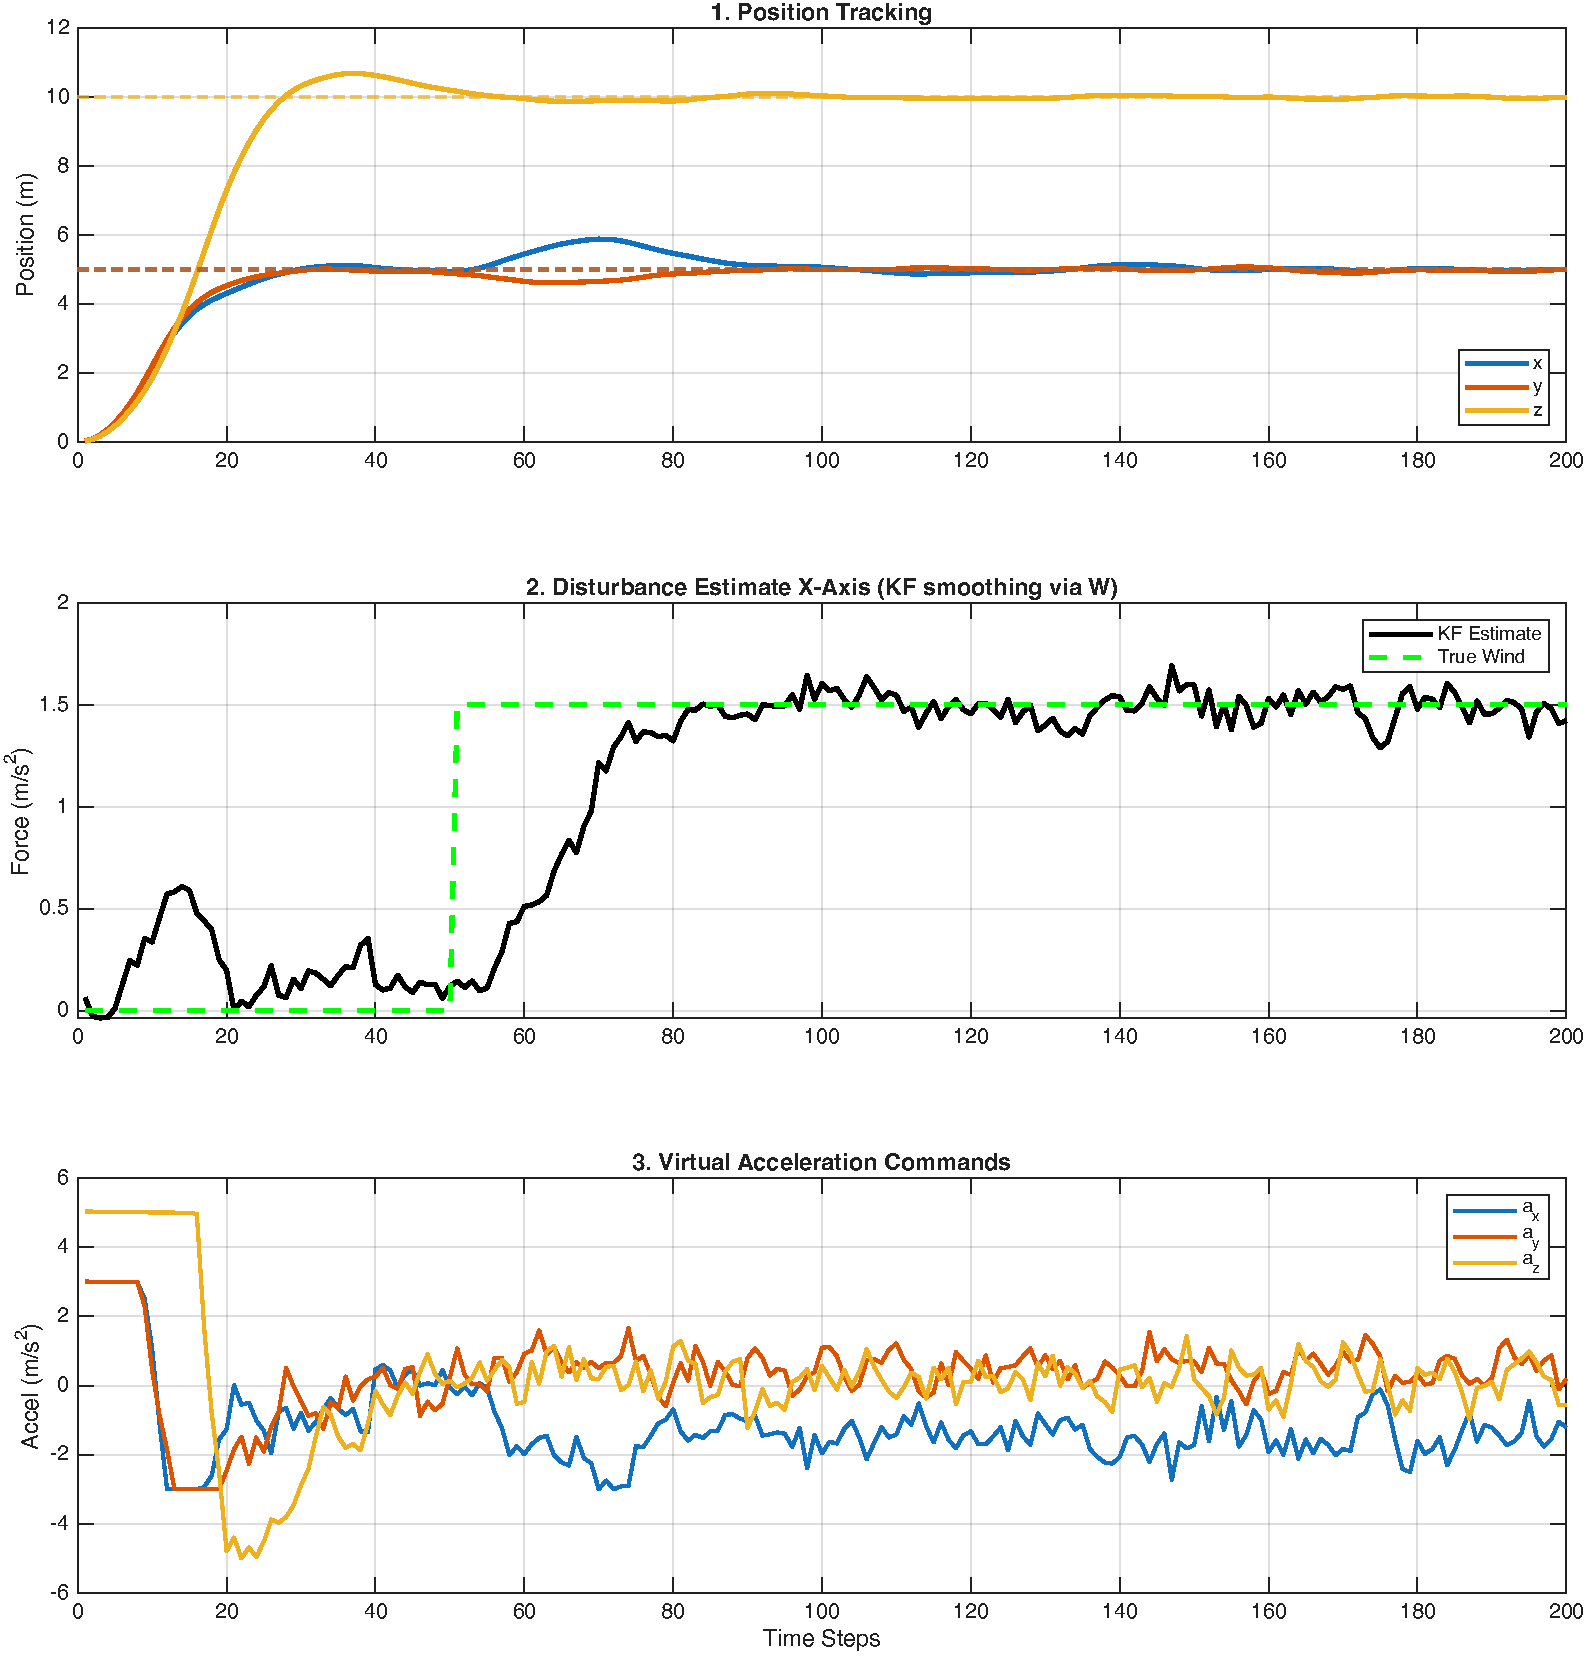
\includegraphics[width=0.9\linewidth]{Figures/Quadrotor_MPC.pdf}
		\captionof{figure}{\textbf{Simulation results: offset-free MPC on a nonlinear quadrotor.} \textbf{Top:} Position tracking. The quadrotor tracks the reference setpoint \([5,5,10]\) m. At \(t=50\) s, a step wind disturbance is applied in the horizontal plane; the trajectory deviates transiently and then returns to the reference with negligible steady-state error. \textbf{Middle:} Disturbance estimation using Kalman Filter. The  estimate converges towards the true wind disturbance. \textbf{Bottom:} Virtual control inputs. After the wind disturbance is applied, the controller settles to non-zero steady virtual accelerations that counteract the wind and maintain the reference position.}
		\label{fig:quad_mpc_result}

	
	\begin{lstlisting}[language=Matlab]
clear; clc; close all;

%% 1. System & Linear Model
g = 9.81; m = 1.0; dt = 0.1;
Ac = [zeros(3,3) eye(3); zeros(3,3) zeros(3,3)];
Bc = [zeros(3,3); eye(3)];
Cc = [eye(3), zeros(3,3)];
sys_d = c2d(ss(Ac, Bc, Cc, 0), dt, 'zoh');
A = sys_d.A; B = sys_d.B; C = sys_d.C;
nx = 6; nu = 3; ny = 3;

%% 2. Augmented Observer
Bw = B;
A_aug = [A, Bw; zeros(3,nx), eye(3)];
B_aug = [B; zeros(3,nu)];
C_aug = [C, zeros(3,3)];

% --- KEY TUNING ---
% W(1:6,1:6)  : process noise on physical states  (keep small)
% W(7:9,7:9)  : process noise on disturbance states
%   LOWER  -> Kalman gain for d is small -> slow update -> implicit LPF
%   HIGHER -> fast disturbance tracking  -> noisier estimate
W = diag([1e-3*ones(1,6), 5e-3*ones(1,3)]);   
V = 1e-2 * eye(3);                              

[P_obs,~,~] = dare(A_aug', C_aug', W, V);
L = P_obs * C_aug' / (C_aug * P_obs * C_aug' + V);

%% 3. Target Calculator
M_target = [eye(nx)-A, -B; C, zeros(ny,nu)];
P_target = pinv(M_target);

%% 4. MPC Formulation (Deviation Form)
N = 50;
Q = diag([20 20 40, 1 1 1]);
R = diag([2 2 2]);
rho = 1e4;
[P_term,~,~] = dare(A, B, Q, R);

du    = sdpvar(nu, N, 'full');
dx    = sdpvar(nx, N+1, 'full');
slack = sdpvar(nu, N, 'full');
x_hat = sdpvar(nx, 1);
x_ss  = sdpvar(nx, 1);
u_ss  = sdpvar(nu, 1);

obj  = 0;
cons = [dx(:,1) == x_hat - x_ss];
for k = 1:N
	cons = [cons, dx(:,k+1) == A*dx(:,k) + B*du(:,k)];
	obj  = obj + dx(:,k)'*Q*dx(:,k) + du(:,k)'*R*du(:,k) + rho*norm(slack(:,k),2)^2;
	u_abs = du(:,k) + u_ss;
	cons = [cons, -3 - slack(1:2,k) <= u_abs(1:2) <= 3 + slack(1:2,k)];
	cons = [cons, -5 - slack(3,k)   <= u_abs(3)   <= 5 + slack(3,k)];
	cons = [cons, slack(:,k) >= 0];
end
obj = obj + dx(:,N+1)'*P_term*dx(:,N+1);
ops = sdpsettings('solver','quadprog','verbose',0);
controller = optimizer(cons, obj, ops, {x_hat, x_ss, u_ss}, du(:,1));

%% 5. Simulation Loop
T_sim      = 200;
x_true     = zeros(6,1);
u_applied  = zeros(3,1);
z_est      = zeros(9,1);
wind_force = [0;0;0];
ref        = [5; 5; 10];

log_x      = zeros(3, T_sim);
log_u      = zeros(3, T_sim);
log_d      = zeros(3, T_sim);
log_d_true = zeros(3, T_sim);

for t = 1:T_sim
	if t > 50, 
		wind_force = [1.5; -0.5; 0]; 
	end

	% A. Measure & Estimate
	y_meas = C*x_true + sqrt(0.01)*randn(3,1);
	z_pred = A_aug*z_est + B_aug*u_applied;
	y_pred = C_aug*z_pred;
	z_est  = z_pred + L*(y_meas - y_pred);
	
	x_hat_val = z_est(1:6);
	d_hat     = z_est(7:9);   
	
	% B. Calculate Targets
	rhs      = [Bw * d_hat; ref];
	ss_sol   = P_target * rhs;
	x_target = ss_sol(1:nx);
	u_target = ss_sol(nx+1:end);
	
	% C. MPC Solve
	[du_opt, err] = controller{x_hat_val, x_target, u_target};
	if err, 
		du_opt = zeros(3,1); 
	end
	u_mpc = du_opt + u_target;
	
	% D. Nonlinear Mapping & Saturation
	accel_z_total = u_mpc(3) + g;
	Thrust    = m * accel_z_total;
	theta_cmd = max(-0.5, min(0.5,  u_mpc(1) / g));
	phi_cmd   = max(-0.5, min(0.5, -u_mpc(2) / g));
	Thrust    = max(0,    min(20,   Thrust));
	u_phys    = [phi_cmd; theta_cmd; Thrust];
	
	% E. Plant Update (Nonlinear)
	x_true    = rk4_step(@quadrotor_dyn, x_true, u_phys, wind_force, dt, m, g);
	u_applied = u_mpc;
	
	log_x(:,t)      = x_true(1:3);
	log_u(:,t)      = u_mpc;
	log_d(:,t)      = d_hat;
	log_d_true(:,t) = wind_force;
end

%% Plotting
t_vec = 1:T_sim;
figure('Color','w','Position',[100 100 800 800]);

subplot(3,1,1);
h = plot(t_vec, log_x, 'LineWidth', 2); hold on;
clr = get(gca,'ColorOrder');
yline(ref(1),'--','Color',clr(1,:),'LineWidth',1.5);
yline(ref(2),'--','Color',clr(2,:),'LineWidth',1.5);
yline(ref(3),'--','Color',clr(3,:),'LineWidth',1.5);
grid on; ylabel('Position (m)');
title('1. Position Tracking');
legend(h,{'x','y','z'},'Location','SouthEast');

subplot(3,1,2);
plot(t_vec, log_d(1,:),      'k',  'LineWidth', 2); hold on;
plot(t_vec, log_d_true(1,:), 'g--','LineWidth', 2);
grid on; ylabel('Force (m/s^2)');
title('2. Disturbance Estimate X-Axis (KF smoothing via W)');
legend('KF Estimate','True Wind');

subplot(3,1,3);
plot(t_vec, log_u, 'LineWidth', 1.5);
legend('a_x','a_y','a_z');
grid on; title('3. Virtual Acceleration Commands');
ylabel('Accel (m/s^2)'); xlabel('Time Steps');

%% Helper Functions
function x_next = rk4_step(fun, x, u, w, dt, m, g)
	k1 = fun(x,           u, w, m, g);
	k2 = fun(x+0.5*dt*k1, u, w, m, g);
	k3 = fun(x+0.5*dt*k2, u, w, m, g);
	k4 = fun(x+dt*k3,     u, w, m, g);
	x_next = x + (dt/6)*(k1 + 2*k2 + 2*k3 + k4);
end

function dxdt = quadrotor_dyn(x, u, w, m, g)
	phi = u(1); theta = u(2); T = u(3);
	Fx  = T*(cos(phi)*sin(theta));
	Fy  = T*(-sin(phi));
	Fz  = T*(cos(phi)*cos(theta));
	ax  = (Fx + w(1))/m;
	ay  = (Fy + w(2))/m;
	az  = (Fz + w(3))/m - g;
	dxdt = [x(4:6); ax; ay; az];
end

	\end{lstlisting}
\end{examplebox}





\begin{examplebox}{Single-zone building heating with economic offset-free MPC}
We consider a heated office room ($\sim$50~m$^2$) whose thermal dynamics
are described by a three-state physically derived RC model discretised at
$T_s = 1800\,\text{s}$ (30~min) via the matrix exponential.
The states are
\[
x_k = \begin{bmatrix} T_{\mathrm{air},k} \\ T_{w,\mathrm{in},k} \\ T_{w,\mathrm{out},k} \end{bmatrix}\!,
\]
representing indoor air temperature, inner wall layer temperature, and
outer wall layer temperature (all in $^\circ$C).
The discrete-time model is
\[
x_{k+1} = A x_k + B u_k + E\,T_{\mathrm{amb},k}
+ B_{\mathrm{sol}}\,\varphi_{\mathrm{sol},k}
+ B_w\,d_k,
\qquad
y_k = C x_k,
\]
where $u_k \in [0, 2000]$~W is the heater power,
$T_{\mathrm{amb},k}$ ($^\circ$C) is the \emph{measured} outdoor temperature,
$\varphi_{\mathrm{sol},k}$ (W/m$^2$) is the \emph{measured} solar
irradiance (both treated as known feedforwards), and $d_k$
($^\circ$C/step) is an \emph{unmeasured} scaled disturbance representing
occupancy and internal heat gains. The output
$y_k = 0.56\,T_{\mathrm{air},k} + 0.44\,T_{w,\mathrm{in},k}$
is the operative temperature (ISO~7726), measured with noise standard
deviation $\sigma_v = 0.1\,^\circ$C.

The pre-computed discrete model matrices are
\begin{align*}
	A &= \begin{bmatrix} 0.8753 & 0.1102 & 0.0004 \\ 0.0275 & 0.9649 & 0.0073 \\ 0.0001 & 0.0049 & 0.9851 \end{bmatrix}, \\[6pt]
	B &= \begin{bmatrix} 7.91\times10^{-4} \\ 1.00\times10^{-4} \\ 0 \end{bmatrix}\!, \quad
	E  = \begin{bmatrix} 0.01404 \\ 0.00025 \\ 0.00993 \end{bmatrix}\!, \quad
	B_{\mathrm{sol}} = \begin{bmatrix} 9.04\times10^{-6} \\ 1.43\times10^{-6} \\ 3.47\times10^{-4} \end{bmatrix}\!, \\[6pt]
	B_w &= \begin{bmatrix} 1.7647 \\ 0.0267 \\ 0 \end{bmatrix}\!, \quad
	C  = \begin{bmatrix} 0.56 & 0.44 & 0 \end{bmatrix}.
\end{align*}

\medskip
\textbf{Exogenous profiles (48-hour winter scenario):}
\begin{itemize}
	\item \textbf{Outdoor temperature} $(T_{\mathrm{amb},k})$:
	\[
	T_{\mathrm{amb},k} = 5 + 6\sin\!\left(\tfrac{2\pi(t_k-14)}{24}\right) + 0.5\,\eta_k,
	\]
	ranging nominally between $-1\,^\circ$C and $11\,^\circ$C; treated as
	a known feedforward.
	
	\item \textbf{Solar irradiance} $(\varphi_{\mathrm{sol},k})$:
	\[
	\varphi_{\mathrm{sol},k} = \max\!\left(0,\; 600\sin\!\left(\tfrac{\pi(\mathrm{mod}(t_k,24)-8)}{9}\right)\right),
	\]
	treated as a known feedforward.
	
	\item \textbf{Occupancy disturbance} $(d_k)$: an effective scaled thermal
	disturbance,
	\[
	d_k = \begin{cases} 0.191\,^\circ\text{C/step} & 08{:}00 \le \mathrm{time}(t_k) < 18{:}00, \\ 0 & \text{otherwise,} \end{cases}
	\]
	corresponding to 300~W of internal gains; \emph{unknown} to the
	controller and estimated by the Kalman filter.
	
	\item \textbf{Electricity price} $(p_k)$:
	\[
	p_k = \begin{cases} 0.28\,\pounds/\text{kWh} & 07{:}00 \le \mathrm{time}(t_k) < 22{:}00, \\ 0.05\,\pounds/\text{kWh} & \text{otherwise.} \end{cases}
	\]
\end{itemize}

\textbf{Time-varying comfort bounds:}
\[
[y_{\min,k},\,y_{\max,k}] = \begin{cases} [20,\,23]\,^\circ\text{C} & \text{daytime }(07{:}00\text{--}22{:}00), \\ [15,\,26]\,^\circ\text{C} & \text{night-time.}\end{cases}
\]

\medskip
\textbf{Control architecture (three layers):}

\begin{enumerate}
	
	\item \textbf{Augmented Kalman observer.}
	The disturbance is appended to the state as a random walk,
	$z_k = [x_k^\top,\, d_k]^\top$, giving the augmented model
	\[
	z_{k+1} =
	\begin{bmatrix} A & B_w \\ 0 & 1 \end{bmatrix} z_k
	+ \begin{bmatrix} B \\ 0 \end{bmatrix} u_k
	+ \begin{bmatrix} E \\ 0 \end{bmatrix} T_{\mathrm{amb},k}
	+ \begin{bmatrix} B_{\mathrm{sol}} \\ 0 \end{bmatrix} \varphi_{\mathrm{sol},k},
	\]
	\[
	y_k = [C,\;0]\,z_k + v_k.
	\]
	 The process noise covariance is selected as
	$W = \mathrm{diag}(10^{-3},10^{-3},10^{-3},\,(0.01)^2)$
	is directly interpretable: $\sqrt{W_d}=0.01\,^\circ$C/step
	represents the expected occupancy change between sampling instants.
	The steady-state Kalman gain $L$ is obtained from the DARE with
	measurement noise variance $V=0.01$.
	
	\item \textbf{Economic steady-state target calculator.}
	At each step, the following QP selects an economically optimal
	steady-state pair $(x_{ss}, u_{ss})$:
	\begin{align*}
		\min_{x_{ss},u_{ss},\epsilon_{ss}} \quad
		& p_k\,u_{ss} + 10^4\,\epsilon_{ss}^2 \\
		\text{s.t.} \quad
		& x_{ss} = A x_{ss} + B u_{ss}
		+ E T_{\mathrm{amb},k}
		+ B_{\mathrm{sol}}\varphi_{\mathrm{sol},k}
		+ B_w \hat d_k, \\
		& y_{\min,k}-\epsilon_{ss} \le C x_{ss} \le y_{\max,k}+\epsilon_{ss},
		\quad 0 \le u_{ss} \le 2000,\quad \epsilon_{ss}\ge 0.
	\end{align*}
	
	\item \textbf{Economic MPC regulator with price preview.}
	Defining $\tilde x_i = x_i - x_{ss}$, $\tilde u_i = u_i - u_{ss}$,
	the regulator solves over a horizon $N=24$ (12~hours):
	\begin{align*}
		\min_{\tilde u,\epsilon} \quad &
		\sum_{i=0}^{N-1}\!\Bigl(
		\|\tilde x_{i+1}\|_Q^2
		+\beta\,p_{k+i}\,(\tilde u_i+u_{ss})\tfrac{T_s}{3600}
		+\rho\,\epsilon_i^2
		\Bigr) + \|\tilde x_N\|_P^2 \\
		\text{s.t.} \quad
		& \tilde x_0 = \hat x_k - x_{ss}, \\
		& \tilde x_{i+1} = A\tilde x_i + B\tilde u_i, \\
		& 0 \le \tilde u_i + u_{ss} \le 2000, \\
		& y_{\min,k+i}-\epsilon_i \le C(\tilde x_{i+1}+x_{ss}) \le y_{\max,k+i}+\epsilon_i,
		\quad \epsilon_i\ge 0,
	\end{align*}
	with $Q=\mathrm{diag}(5,2,1)$, $\beta=6$, $\rho=10^7$, and
	$P$ from the DARE.
	The term $\beta p_{k+i}(\tilde u_i+u_{ss})(T_s/3600)$ is the actual
	energy expenditure in pounds at future step $k+i$.
	The penalty hierarchy
	$\rho \gg \beta\,p_{\max}\,u_{\max}\,(T_s/3600)$,
	i.e.\ $10^7 \gg 1680$, ensures comfort violations are never
	preferred over heating.
\end{enumerate}

\textbf{MATLAB implementation:} The plotting section is omitted below.

\begin{lstlisting}[language=MATLAB]
	clear; clc; close all; rng(1);
	
	%% 1. Pre-computed Discrete Model (3R2C, ZOH, Ts = 1800 s)
	%    x = [T_air; T_w_in; T_w_out] (degC)
	%    u = heater power (W),  u in [0, 2000]

	Ts = 1800;
	A  = [	0.8753, 0.1102, 0.0004;
				0.0275, 0.9649, 0.0073;
				0.0001, 0.0049, 0.9851];
	B      = [7.91e-4; 1.00e-4; 0      ];
	E      = [0.01404; 0.00025; 0.00993];   
	Bsol   = [9.04e-6; 1.43e-6; 3.47e-4];  
	Bw     = [1.7647;  0.0267;  0      ];   
	C      = [0.56, 0.44, 0];               
	
	nx = 3;  nu = 1;  ny = 1; u_min = 0;  u_max = 2000;
	
	%% 2. Augmented Kalman Observer
	%    z = [x; d],  random-walk disturbance model
	
	A_aug = [A, Bw; zeros(1,nx), 1];
	B_aug = [B; 0];  E_aug = [E; 0];  Bsol_aug = [Bsol; 0];
	C_aug = [C, 0];
	
	W_kf = diag([1e-3, 1e-3, 1e-3, (0.01)^2]);  
	V_kf = 0.1^2;
	
	[P_kf,~,~] = dare(A_aug', C_aug', W_kf, V_kf);
	L_kf = P_kf*C_aug'/(C_aug*P_kf*C_aug' + V_kf);
	
	%% 3. Economic Steady-State Target Calculator
	price_in   = sdpvar(1);  d_in     = sdpvar(1);
	T_amb_in   = sdpvar(1);  phi_in   = sdpvar(1);
	y_min_in   = sdpvar(1);  y_max_in = sdpvar(1);
	xs = sdpvar(nx,1);  us = sdpvar(nu,1);  ss_slack = sdpvar(1);
	
	ss_cons = [xs == A*xs + B*us + E*T_amb_in + Bsol*phi_in + Bw*d_in, ...
	y_min_in - ss_slack <= C*xs <= y_max_in + ss_slack, ...
	u_min <= us <= u_max, ss_slack >= 0];
	ss_obj  = price_in*us + 1e4*ss_slack^2;
	
	target_calc = optimizer(ss_cons, ss_obj, ...
	sdpsettings('solver','quadprog','verbose',0), ...
	{price_in, d_in, T_amb_in, phi_in, y_min_in, y_max_in}, [xs; us]);
	
	%% 4. Economic MPC Regulator with Price Preview (N = 24, horizon = 12 h)
	%    Stage cost: ||x_tilde||_Q^2 + beta*price*u*(Ts/3600) + rho*slack^2
	%    Penalty hierarchy: rho >> beta*p_max*u_max*(Ts/3600)
	%    i.e.  1e7 >> 10*0.28*2000*0.5 = 2800
	N = 24;  Q = diag([5,2,1]);  rho = 1e7;  beta = 6;
	[P_term,~,~] = dare(A, B, Q, 1e-3);
	
	du        = sdpvar(nu,N,'full');   dx    = sdpvar(nx,N+1,'full');
	mpc_slack = sdpvar(1,N,'full');
	xhat_in   = sdpvar(nx,1);  xss_in = sdpvar(nx,1);  uss_in = sdpvar(nu,1);
	Ymin_seq  = sdpvar(1,N,'full');    Ymax_seq  = sdpvar(1,N,'full');
	Price_seq = sdpvar(1,N,'full');
	
	mpc_obj  = 0;
	mpc_cons = [dx(:,1) == xhat_in - xss_in];
	for i = 1:N
		u_abs    = du(:,i) + uss_in;
		x_pred_i = dx(:,i+1) + xss_in;
		mpc_cons = [mpc_cons, ...
		dx(:,i+1) == A*dx(:,i) + B*du(:,i), ...
		u_min <= u_abs <= u_max, ...
		Ymin_seq(i)-mpc_slack(i) <= C*x_pred_i <= Ymax_seq(i)+mpc_slack(i), ...
		mpc_slack(i) >= 0];
		mpc_obj = mpc_obj + dx(:,i)'*Q*dx(:,i) ...
		+ beta*Price_seq(i)*u_abs*(Ts/3600) ...
		+ rho*mpc_slack(i)^2;
	end
	mpc_obj = mpc_obj + dx(:,N+1)'*P_term*dx(:,N+1);
	
	mpc_reg = optimizer(mpc_cons, mpc_obj, ...
	sdpsettings('solver','quadprog','verbose',0), ...
	{xhat_in,xss_in,uss_in,Ymin_seq,Ymax_seq,Price_seq}, du(:,1));
	
	%% 5. Exogenous Profiles (48-hour simulation)
	N_sim   = 48*(3600/Ts);
	t_hours = (0:N_sim+N)*(Ts/3600);
	
	T_amb_profile = 5 + 6*sin(2*pi*(t_hours-14)/24) + 0.5*randn(size(t_hours));
	Solar_profile = max(0, 600*sin(pi*(mod(t_hours,24)-8)/9));
	Elec_Price    = 0.05*ones(size(t_hours));
	day_mask      = mod(t_hours,24) >= 7 & mod(t_hours,24) < 22;
	Elec_Price(day_mask) = 0.28;
	Tmin_profile  = 15*ones(size(t_hours));  Tmin_profile(day_mask) = 20;
	Tmax_profile  = 26*ones(size(t_hours));  Tmax_profile(day_mask) = 23;
	% True occupancy: 300 W = 0.191 degC/step (unknown to controller)
	d_occ_profile = 0.191*double(mod(t_hours,24) >= 8 & mod(t_hours,24) < 18);
	
	%% 6. Closed-Loop Simulation
	x_true = [19; 17; 10];  z_est = [19; 17; 10; 0];  u_prev = 0;
	
	log_Top  = zeros(1,N_sim);  log_Tmeas = zeros(1,N_sim);
	log_u    = zeros(1,N_sim);  log_d_est = zeros(1,N_sim);
	log_dtrue= zeros(1,N_sim);  log_price = zeros(1,N_sim);
	log_Tmin = zeros(1,N_sim);  log_Tmax  = zeros(1,N_sim);
	log_cost = zeros(1,N_sim);
	
	for k = 1:N_sim
		T_amb_k   = T_amb_profile(k);
		phi_sol_k = Solar_profile(k);
		y_meas    = C*x_true + sqrt(V_kf)*randn;
		
		% KF predict & correct (current-step feedforwards)
		if k == 1,  
			z_pred = z_est;
		else
			z_pred = A_aug*z_est + B_aug*u_prev ...
		+ E_aug*T_amb_k + Bsol_aug*phi_sol_k;
		end
		z_est = z_pred + L_kf*(y_meas - C_aug*z_pred);
		x_hat = z_est(1:nx);  d_hat = z_est(end);
		
		% Economic target
		y_min = Tmin_profile(k);  y_max = Tmax_profile(k);
		[ss_sol, err_ss] = target_calc{Elec_Price(k),d_hat,T_amb_k,phi_sol_k,y_min,y_max};
		if err_ss ~= 0,  
			x_ss = x_hat; 	u_ss = u_prev;
		else,  
			ss_sol=full(ss_sol); x_ss=ss_sol(1:nx); u_ss=ss_sol(nx+1);
		end
		% Economic MPC with N-step price preview
		[du_opt, err_mpc] = mpc_reg{x_hat, x_ss, u_ss, ...
				Tmin_profile(k+1:k+N), Tmax_profile(k+1:k+N), Elec_Price(k+1:k+N)};
		if err_mpc ~= 0,  
			du_opt = 0;  
		else,  
			du_opt = full(du_opt);  
		end
		u_prev = min(max(u_ss + du_opt, u_min), u_max);
	
		% Plant update (true occupancy unknown to controller)
		x_true = A*x_true + B*u_prev + E*T_amb_k ...
		+ Bsol*phi_sol_k + Bw*d_occ_profile(k);
		
		% Logging
		log_Top(k)  = C*x_true;   log_Tmeas(k) = y_meas;
		log_u(k)    = u_prev;      log_d_est(k) = d_hat;
		log_dtrue(k)= d_occ_profile(k);
		log_Tmin(k) = y_min;       log_Tmax(k)  = y_max;
		log_price(k)= Elec_Price(k);
		log_cost(k) = Elec_Price(k)*u_prev*(Ts/3600)/1000;  % GBP per step
	end
	fprintf('Total heating cost: GBP %.3f\n', sum(log_cost));
	
	% Visualisation is omitted for brevity
\end{lstlisting}

	\centering
	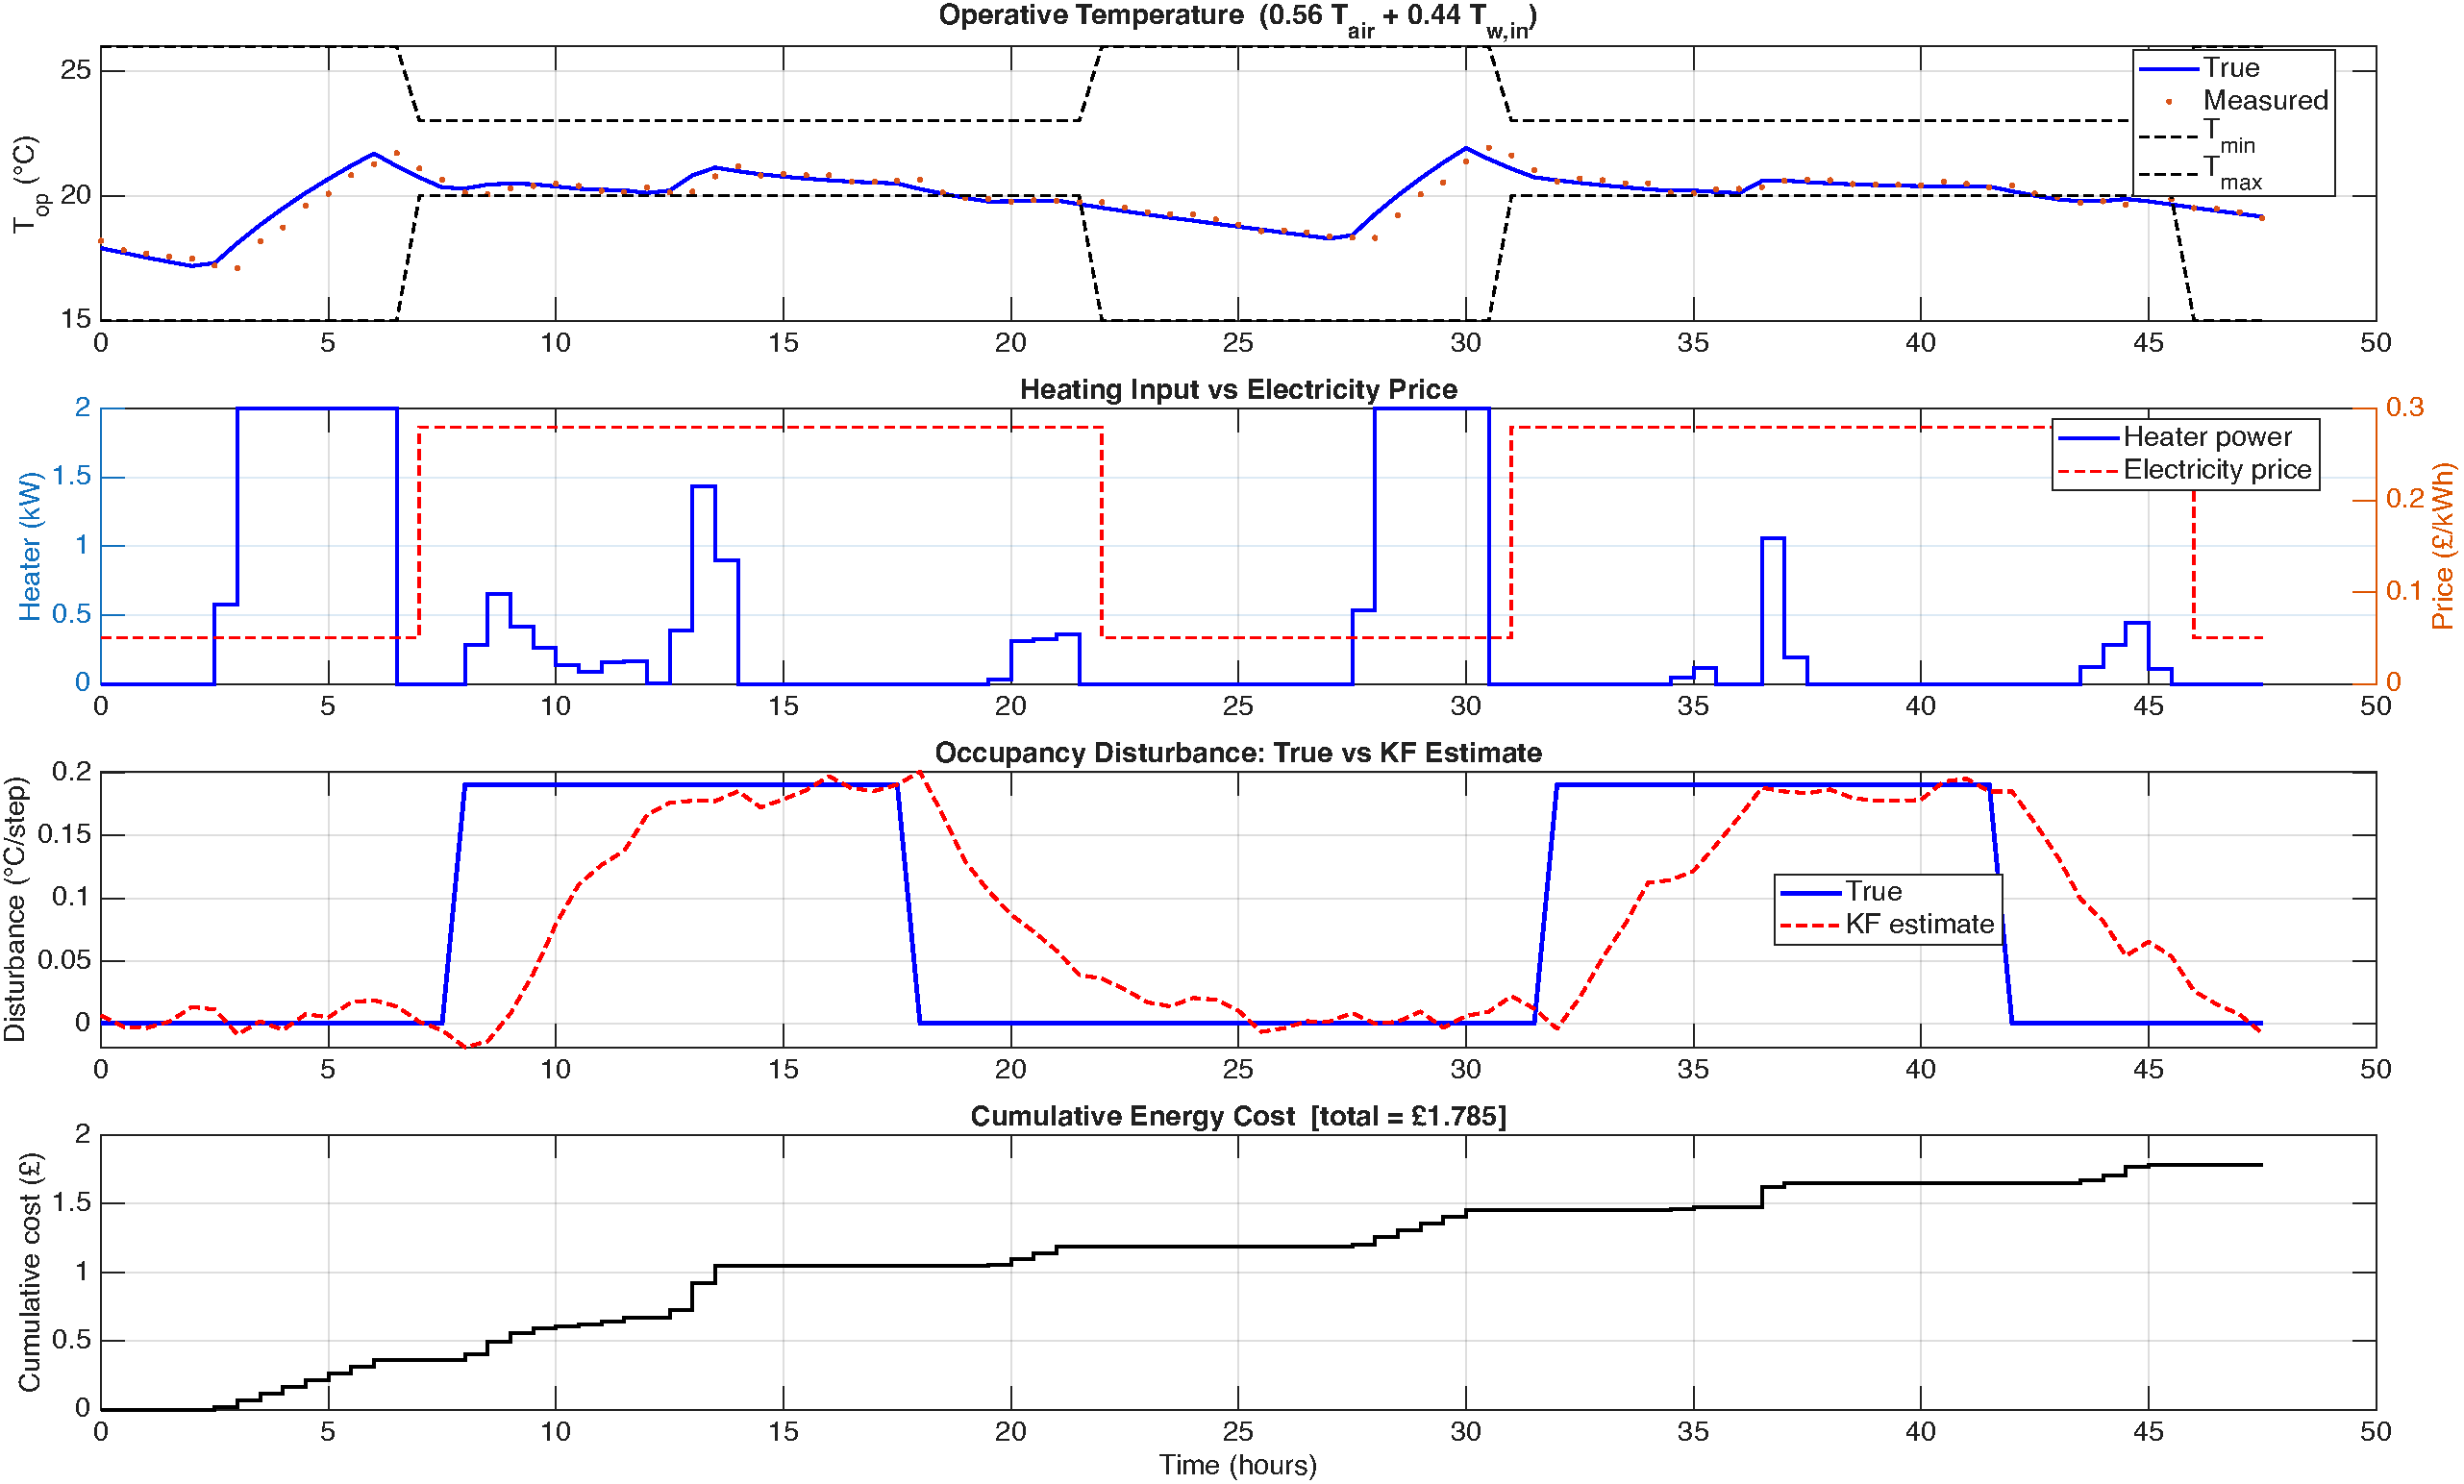
\includegraphics[width=0.9\linewidth]{Figures/hvac.pdf}
	\captionof{figure}{Closed-loop performance of the economic offset-free MPC for the
		single-zone building heating example over a 48-hour simulation.
		\textit{Top:} Operative temperature tracking the time-varying comfort
		region; the controller pre-heats during the cheap off-peak window before
		07:00 and reduces heating during the expensive daytime tariff.
		\textit{Second:} Heater power overlaid with the electricity price;
		the load-shifting behaviour is clearly visible.
		\textit{Third:} True occupancy disturbance versus the Kalman filter
		estimate; convergence is fast because $CB_w = 1$.
		\textit{Bottom:} Cumulative energy cost in GBP over the 48-hour horizon.}
	\label{fig:singlezone2}

\end{examplebox}

% ===================================================================
%  Example: Offset-free MPC for a 3-DOF Articulated Robot Manipulator
%  Drop this file into your chapter via \input{Example_3DOF_MPC}
%  Requires the preamble from Main.tex (tcolorbox, listings, tikz, etc.)
% ===================================================================

\begin{examplebox}{Offset-free MPC of a 3-DOF Articulated Robot Manipulator}
	
	% -------------------------------------------------------------------
	%  PART 1 — Problem Description
	% -------------------------------------------------------------------
	\textbf{\textsf{Problem Description}}
	
	Consider a three-degree-of-freedom (3-DOF) \emph{RRR} articulated robot manipulator
	operating in three-dimensional space. The three revolute joints are arranged as follows:
	joint~1 rotates about the vertical ($z$) axis (base yaw), whilst joints~2 and~3 rotate
	about parallel horizontal ($y$) axes (shoulder and elbow pitch, respectively). This
	configuration is representative of the positioning structure found in industrial serial
	manipulators.
	
	The control objective is to track piecewise-constant joint-angle references
	$r(t) \in \mathbb{R}^{3}$ in the presence of persistent disturbances (joint friction
	and unexpected payload changes) whilst respecting hard torque limits and soft joint-angle
	limits. An offset-free MPC strategy based on computed-torque feedback linearisation and
	an augmented Kalman filter (AKF) is employed.
	
	% -------------------------------------------------------------------
	%  PART 2 — Kinematic Configuration (TikZ)
	% -------------------------------------------------------------------
	\vspace{0.5em}
	\textbf{\textsf{Kinematic Configuration}}
	
	Figure~\ref{fig:3dof_arm} shows the side-view projection of the arm and the
	definition of the joint angles $q_1$, $q_2$, and $q_3$. The base yaw axis
	is perpendicular to the plane of the figure.
	
	\begin{figure}[H]
		\centering
		\begin{tikzpicture}[
			every node/.style={font=\small\sffamily},
			joint/.style={circle, draw=excolor, fill=exback, thick, minimum size=7pt, inner sep=0pt},
			link/.style={draw=black!70, line width=2.5pt, line cap=round},
			ground/.style={pattern=north east lines, pattern color=black!40, draw=black!60}
			]
			
			% --- Ground / base pedestal ---
			\fill[ground] (-0.6,-0.55) rectangle (0.6,-0.3);
			\draw[thick] (-0.6,-0.3) -- (0.6,-0.3);
			
			% --- Link lengths (display scale) ---
			% a2 = 0.45 m  →  3.6 units
			% a3 = 0.35 m  →  2.8 units
			% scale factor 8
			
			% --- Joint angles (display) ---
			\pgfmathsetmacro{\qTwo}{55}
			\pgfmathsetmacro{\qThree}{-65}
			
			% --- Joint 1 (origin, base yaw shown as cross-section circle) ---
			\coordinate (J1) at (0,0);
			\draw[link] (0,-0.3) -- (J1);
			\node[joint, minimum size=10pt] at (J1) {};
			\node[above right=1pt] at (J1) {$q_1$ (yaw)};
			
			% Yaw axis indicator
			\draw[thick, excolor] (J1) circle (4pt);
			\fill[excolor] (J1) circle (1.5pt);
			
			% --- Upper arm (Link 2) ---
			\coordinate (J2) at ($(J1) + (\qTwo:3.6)$);
			\draw[link, excolor!70!black] (J1) -- (J2);
			
			% Angle arc q2
			\draw[->, excolor, thick] (0.9,0) arc[start angle=0, end angle=\qTwo, radius=0.9];
			\node[right] at (1.0,0.7) {$q_2$};
			
			% COM marker link 2
			\coordinate (COM2) at ($(J1)!0.5!(J2)$);
			\fill[black!40] (COM2) circle (2.5pt);
			\node[above left, xshift=-2pt] at (COM2) {\footnotesize $l_{c2}$};
			
			% --- Joint 2 ---
			\node[joint] at (J2) {};
			\node[above right=1pt] at (J2) {$q_2$ (shoulder)};
			
			% --- Forearm (Link 3) ---
			\pgfmathsetmacro{\absThree}{\qTwo + \qThree}
			\coordinate (J3) at ($(J2) + (\absThree:2.8)$);
			\draw[link, excolor!40!black] (J2) -- (J3);
			
			% Angle arc q3
			\pgfmathsetmacro{\arcStart}{\qTwo}
			\pgfmathsetmacro{\arcEnd}{\qTwo + \qThree}
			\draw[->, excolor!60!black, thick]
			($(J2) + (\arcStart:0.8)$) arc[start angle=\arcStart, end angle=\arcEnd, radius=0.8];
			\node[right=4pt] at ($(J2) + (\arcStart:0.9)$) {$q_3$};
			
			% COM marker link 3
			\coordinate (COM3) at ($(J2)!0.48!(J3)$);
			\fill[black!40] (COM3) circle (2.5pt);
			\node[below right, xshift=2pt] at (COM3) {\footnotesize $l_{c3}$};
			
			% --- End-effector ---
			\node[joint, minimum size=5pt, fill=excolor] at (J3) {};
			\node[right=3pt] at (J3) {end-effector};
			
			% --- Dimension lines ---
			\draw[<->, gray, thin]
			($(J1)!0.08!(J2) + (-70:0.25)$) -- ($(J1)!0.92!(J2) + (-70:0.25)$)
			node[midway, below, gray] {$a_2 = 0.45\,\mathrm{m}$};
			
			\draw[<->, gray, thin]
			($(J2)!0.08!(J3) + ({\absThree-90}:0.25)$) -- ($(J2)!0.92!(J3) + ({\absThree-90}:0.25)$)
			node[midway, below, gray] {$a_3 = 0.35\,\mathrm{m}$};
			
			% --- Legend ---
			\draw[link, excolor!70!black, line width=1.5pt] (5.0,1.8) -- (5.4,1.8);
			\node[right] at (5.45,1.8) {\small Upper arm (Link 2)};
			
			\draw[link, excolor!40!black, line width=1.5pt] (5.0,1.2) -- (5.4,1.2);
			\node[right] at (5.45,1.2) {\small Forearm (Link 3)};
			
			\node[joint, minimum size=7pt] at (5.2, 0.6) {};
			\node[right] at (5.45, 0.6) {\small Revolute joint};
			
		\end{tikzpicture}
		\caption{Side-view projection of the 3-DOF RRR articulated arm.
			Joint~1 (base yaw) is perpendicular to the page; joints~2 and~3
			(shoulder and elbow pitch) lie in the plane shown.}
		\label{fig:3dof_arm}
	\end{figure}
	
	% -------------------------------------------------------------------
	%  PART 3 — Robot Parameters
	% -------------------------------------------------------------------
	\textbf{\textsf{Physical Parameters}}
	
	
	\begin{center}
		\captionof{table}{Parameters used in the simulation.}
		\begin{tabular}{llcc}
			\toprule
			Symbol & Description & Value & Unit \\
			\midrule
			$I_{z1}$  & Base yaw inertia (joint 1)         & 1.50  & kg\,m$^{2}$ \\
			$m_2$     & Mass of upper arm (link 2)          & 6.00  & kg          \\
			$a_2$     & Length of upper arm                  & 0.45  & m           \\
			$l_{c2}$  & COM distance from joint 2           & 0.22  & m           \\
			$I_2$     & Pitch inertia of link 2 about COM   & 0.15  & kg\,m$^{2}$ \\
			$m_3$     & Mass of forearm (link 3)            & 3.50  & kg          \\
			$a_3$     & Length of forearm                    & 0.35  & m           \\
			$l_{c3}$  & COM distance from joint 3           & 0.17  & m           \\
			$I_3$     & Pitch inertia of link 3 about COM   & 0.08  & kg\,m$^{2}$ \\
			$T_s$     & Sampling period                      & 0.02  & s           \\
			\bottomrule
		\end{tabular}
	\end{center}
	
	% -------------------------------------------------------------------
	%  PART 4 — Control Strategy
	% -------------------------------------------------------------------
	\vspace{0.4em}
	\textbf{\textsf{Control Technique: Computed-Torque MPC with Disturbance Observer}}
	
	The full nonlinear robot dynamics are:
	\begin{equation}
		M(q)\,\ddot{q} + Cor(q,\dot{q})\,\dot{q} + G(q) = \tau + d_{\tau},
		\label{eq:robot_dyn}
	\end{equation}
	where $q \in \mathbb{R}^{3}$ are the joint angles, $M(q)$ is the symmetric
	positive-definite inertia matrix, $Cor(q,\dot{q})\dot{q}$ collects Coriolis and
	centrifugal torques, $G(q)$ is the gravity vector, $\tau$ is the applied torque, and
	$d_{\tau} \in \mathbb{R}^{3}$ represents lumped torque-space disturbances
	(friction, payload) in~[Nm].
	
	\emph{Computed-torque (CT) feedback linearisation} is applied by choosing:
	\begin{equation}
		\tau = M(q)\,v + Cor(q,\dot{q})\,\dot{q} + G(q),
		\label{eq:ct_law}
	\end{equation}
	which reduces~\eqref{eq:robot_dyn} to three decoupled double integrators,
	one per joint:
	\begin{equation}
		\ddot{q} = v + \underbrace{M(q)^{-1}\,d_{\tau}}_{\displaystyle d},
		\label{eq:double_int}
	\end{equation}
	where $d \triangleq M(q)^{-1}\,d_{\tau} \in \mathbb{R}^{3}$ is the
	\emph{acceleration-space disturbance}~[rad/s$^{2}$].
	Because the MPC and observer operate entirely in the linearised
	(virtual-acceleration) domain, $d$~is the natural disturbance variable
	for the remainder of the formulation.
	If the physical torque-space disturbance is needed, it can be recovered as
	$\hat{d}_{\tau} = M(q)\,\hat{d}$.
	
	Defining the state $x = [q^{\top},\,\dot{q}^{\top}]^{\top} \in \mathbb{R}^{6}$,
	the linearised continuous-time plant is:
	\begin{equation}
		\dot{x} =
		\underbrace{\begin{bmatrix}0 & I \\ 0 & 0\end{bmatrix}}_{A_c}x +
		\underbrace{\begin{bmatrix}0 \\ I\end{bmatrix}}_{B_c}v, \qquad
		y = \underbrace{\begin{bmatrix}I & 0\end{bmatrix}}_{C}\,x,
		\label{eq:lin_plant}
	\end{equation}
	which is discretised exactly via zero-order hold at $T_s = 0.02$\,s to give
	$(A,\,B,\,C)$. The entire control scheme is shown in Figure~\ref{fig:CTMPC_robot_block_diagram}.
	
	% -------------------------------------------------------------------
	%  PART 5 — MPC Formulation
	% -------------------------------------------------------------------
	\vspace{0.4em}
	\textbf{\textsf{MPC Formulation}}
	
	\emph{Augmented observer for offset-free control.}
	A random-walk model $d_{k+1} = d_k$ for the acceleration-space disturbance
	is appended to the plant state,
	yielding the augmented system $z = [x^{\top},\,d^{\top}]^{\top} \in \mathbb{R}^{9}$:
	\begin{equation}
		\begin{bmatrix}x_{k+1}\\d_{k+1}\end{bmatrix}
		=
		\underbrace{\begin{bmatrix}A & B \\ 0 & I\end{bmatrix}}_{A_{\mathrm{aug}}}
		\begin{bmatrix}x_k\\d_k\end{bmatrix}
		+
		\underbrace{\begin{bmatrix}B\\0\end{bmatrix}}_{B_{\mathrm{aug}}}v_k, \qquad
		y_k =
		\underbrace{\begin{bmatrix}C & 0\end{bmatrix}}_{C_{\mathrm{aug}}}
		\begin{bmatrix}x_k\\d_k\end{bmatrix}.
		\label{eq:aug_sys}
	\end{equation}
	Note that $d$ enters the state equation through $B$ (the same input matrix as $v$),
	confirming that it represents the disturbance in virtual-acceleration
	units~[rad/s$^{2}$], not in torque units~[Nm].
	The observer gain $L$ is obtained from the discrete algebraic Riccati equation
	(DARE) with process noise covariance
	$Q = \mathrm{diag}(10^{-6}I_6,\;10^{-3}I_3)$ and measurement noise
	covariance $R = \sigma_{\mathrm{enc}}^{2}\,I_3$ where
	$\sigma_{\mathrm{enc}} = 0.05^{\circ}$ (encoder standard deviation). The controller can only access the measurements of angular positions, $q$. Therefore, $C=\begin{bmatrix}
	I_{3\times 3} & 0_{3\times 3}
	\end{bmatrix}$
	
	\emph{Target calculator.}
	At steady state, $x_{k+1} = x_k = x_{\mathrm{ss}}$ and $y_{\mathrm{ss}} = r_k$,
	so the pair $(x_{\mathrm{ss}},\,v_{\mathrm{ss}})$ satisfies:
	\begin{equation}
		\begin{bmatrix}I - A & -B \\ C & 0\end{bmatrix}
		\begin{bmatrix}x_{\mathrm{ss}} \\ v_{\mathrm{ss}}\end{bmatrix}
		=
		\begin{bmatrix}B\,\hat{d}_k \\ r_k\end{bmatrix}.
		\label{eq:target}
	\end{equation}
	This ensures that the MPC drives the plant to the reference with zero steady-state
	offset despite the persistent acceleration-space disturbance estimate
	$\hat{d}_k$~[rad/s$^{2}$].
	
	\emph{Deviation-form optimal control problem.}
	Let $\delta x_k = x_k - x_{\mathrm{ss}}$ and $\delta v_k = v_k - v_{\mathrm{ss}}$.
	The QP solved at each sampling instant is:
	\begin{equation}
		\begin{aligned}
			\min_{\{\delta v_k\},\{s_k\}}\;\;
			&\sum_{k=0}^{N-1}\!\left[
			\delta y_k^{\top} Q_y\,\delta y_k
			+ \delta v_k^{\top} R\,\delta v_k
			+ \rho\,s_k^{\top}s_k
			\right]
			+ \delta x_N^{\top} P_N\,\delta x_N \\[4pt]
			\text{subject to}\;\;
			&\delta x_{k+1} = A\,\delta x_k + B\,\delta v_k,
			\quad \delta x_0 = \hat{x}_k - x_{\mathrm{ss}},\\
			&v_{\min} \leq \delta v_k + v_{\mathrm{ss}} \leq v_{\max},\\
			&y_{\min} - s_k \leq C(\delta x_k + x_{\mathrm{ss}}) \leq y_{\max} + s_k,\\
			&s_k \geq 0, \quad k = 0, \ldots, N-1,
		\end{aligned}
		\label{eq:ocp}
	\end{equation}
	where $\delta y_k = C\,\delta x_k$, $P_N$ is the terminal LQR cost matrix (from the
	DARE for $(A,B,Q_{\mathrm{mpc}},R)$), and $s_k \in \mathbb{R}^{3}$ are slack
	variables that soften the joint-angle constraints.
	
	The MPC tuning parameters are summarised in Table~\ref{tab:robot_parameters}.
	
	
	\captionof{table}{Robot parameters.}\label{tab:robot_parameters}
	\begin{center}
		\begin{tabular}{llc}
			\toprule
			Parameter & Description & Value \\
			\midrule
			$N$        & Prediction horizon                        & 15 \\
			$Q_y$      & Output tracking weight                    & $200\,I_3$ \\
			$R$        & Control effort weight                     & $0.1\,I_3$ \\
			$\rho$     & Soft-constraint penalty                   & $10^{6}$ \\
			$v_{\min}$ & Virtual acceleration lower bound          & $-50\,\mathrm{rad/s}^2$ \\
			$v_{\max}$ & Virtual acceleration upper bound          & $+50\,\mathrm{rad/s}^2$ \\
			$y_{\min}$ & Joint angle lower limits                  & $[-170^\circ,\,-90^\circ,\,-135^\circ]^{\top}$ \\
			$y_{\max}$ & Joint angle upper limits                  & $[+170^\circ,\,+90^\circ,\,+135^\circ]^{\top}$ \\
			$\tau_{\max}$ & Actuator torque limits (absolute)      & $[150,\,120,\,60]\,\mathrm{Nm}$ \\
			\bottomrule
		\end{tabular}
	\end{center}
	
	
	\begin{center}
		\begin{tikzpicture}[scale=0.8, transform shape]
			
			\tikzset{
				block/.style={
					draw, rectangle, rounded corners=2pt,
					minimum height=1.4cm, minimum width=2.8cm,
					text width=2.6cm, align=center,
					font=\small\sffamily, line width=0.7pt,
				},
				wideblock/.style={
					draw, rectangle, rounded corners=2pt,
					minimum height=1.6cm, minimum width=3.5cm,
					text width=4cm, align=center,
					font=\small\sffamily, line width=0.7pt,
				},
				smallblock/.style={
					draw, rectangle, rounded corners=2pt,
					minimum height=1.1cm, minimum width=2.2cm,
					text width=2.0cm, align=center,
					font=\footnotesize\sffamily, line width=0.7pt,
				},
				arr/.style={-Stealth, line width=0.65pt},
				sig/.style={font=\footnotesize\sffamily},
				sm/.style={font=\footnotesize},
			}
			
			% =====================================================================
			%  ROW 1 (y=0):  ref -> Target -> MPC -> CT -> Sat
			% =====================================================================
			
			\node[sig] (ref) at (-1, 0) {$r(t)$};
			
			\node[wideblock, fill=targetpurp!10, draw=targetpurp]
			(target) at (3., 0) {%
				\textbf{Target Calculator}\\[2pt]
				{\footnotesize $\begin{bmatrix} I{-}A & -B \\ C & 0 \end{bmatrix}
					\begin{bmatrix} x_\mathrm{ss} \\ u_\mathrm{ss} \end{bmatrix}
					{=} \begin{bmatrix} B\,\hat{d} \\ r \end{bmatrix}$}
			};
			
			\node[block, fill=mpcblue!10, draw=mpcblue]
			(mpc) at (7.8, 0) {%
				\textbf{MPC}\\[2pt]
				{\footnotesize Deviation form}\\[-1pt]
				{\footnotesize $N{=}15,\; Q_y{=}200$}\\[-1pt]
				{\footnotesize $R{=}0.1$}
			};
			
			\node[block, fill=ctgray!10, draw=ctgray]
			(ct) at (12.2, 0) {%
				\textbf{Computed-Torque}\\[2pt]
				{\footnotesize $\tau = M(q)\,v$}\\[-1pt]
				{\footnotesize $+ Cor(q,\dot{q})\dot{q} + G$}
			};
			
			\node[smallblock, fill=satred!10, draw=satred]
			(sat) at (15.6, 0) {%
				\textbf{Saturation}\\[1pt]
				{\footnotesize $|\tau| \leq \tau_{\max}$}
			};
			
			% =====================================================================
			%  ROW 2 (y=-4.5):  AKF --- BackCalc --- Sensor --- Plant
			% =====================================================================
			
			\node[wideblock, fill=obsvorange!10, draw=obsvorange,
			minimum height=1.8cm, minimum width=3.5cm, text width=3.3cm]
			(akf) at (3., -4.5) {%
				\textbf{Augmented Kalman}\\
				\textbf{Filter}\\[2pt]
				{\footnotesize $\hat{z} = [\hat{x};\, \hat{d}]$}\\[-1pt]
				{\footnotesize $\hat{z}^- {=} A_\mathrm{aug}\hat{z} {+} B_\mathrm{aug} v_\mathrm{app}$}\\[-1pt]
				{\footnotesize $\hat{z}^+ {=} \hat{z}^- {+} L(y{-}C_\mathrm{aug}\hat{z}^-)$}
			};
			
			\node[wideblock, fill=ctgray!8, draw=ctgray]
			(backcalc) at (7.7, -4.5) {%
				\textbf{Back-Calc}\\[1pt]
				{\footnotesize $v_\mathrm{app} {=} M^{-1}(\tau_\mathrm{sat}{-}C\dot{q}{-}G)$}
			};
			
			\node[smallblock, fill=sensorgold!10, draw=sensorgold]
			(sensor) at (11.6, -4.5) {%
				\textbf{Encoder}\\[1pt]
				{\footnotesize $y = q + n$}\\[-1pt]
				{\footnotesize $\sigma = 0.05^\circ$}
			};
			
			\node[wideblock, fill=plantgreen!10, draw=plantgreen,
			minimum width=3.2cm, text width=3.0cm]
			(plant) at (15.6, -4.5) {%
				\textbf{Nonlinear Robot}\\[2pt]
				{\footnotesize $M\ddot{q} {+} Cor\dot{q} {+} G= \tau {+} d_\tau(t)$}\\[-1pt]
				{\footnotesize RK4, $T_s{=}0.02\,$s}
			};
			
			% Disturbance input (from below)
			\node[sig] (dist) at (15.6, -6.8) {$d_{\tau}(t)$\; {\tiny friction + payload}};
			
			% =====================================================================
			%  FORWARD PATH  (Row 1, left to right)
			% =====================================================================
			
			\draw[arr] (ref) -- (target)
			node[midway, above, sig] {$r \in \mathbb{R}^3$};
			
			\draw[arr] (target) -- (mpc)
			node[midway, above, sm] {$x_\mathrm{ss},\, u_\mathrm{ss}$};
			
			\draw[arr] (mpc) -- (ct)
			node[midway, above, sm] {$v_\mathrm{opt}$}
			node[midway, below, sig] {\tiny [rad/s$^2$]};
			
			\draw[arr] (ct) -- (sat)
			node[midway, above, sm] {$\tau_\mathrm{cmd}$};
			
			% =====================================================================
			%  Sat -> Plant  (vertical connector between rows)
			% =====================================================================
			
			\draw[arr] (sat.south) -- (plant.north)
			node[midway, right, sm, xshift=2pt] {$\tau_\mathrm{sat}$};
			
			% Disturbance -> Plant
			\draw[arr] (dist) -- (plant.south);
			
			% =====================================================================
			%  ROW 2 FEEDBACK  (right to left)
			% =====================================================================
			
			% Plant -> Sensor  (straight horizontal)
			\draw[arr] (plant.west) -- (sensor.east)
			node[midway, above, sm] {$q,\, \dot{q}$};
			
			% Sensor -> AKF  (route below Row 2 blocks to avoid crossing Back-Calc)
			%   sensor.south -> down -> left -> up -> akf.south
			\draw[arr]
			(sensor.south) -- ++(0, -1.5)
			-- ($(akf.south) + (0., -0.65)$)
			-- ($(akf.south) $)
			node[pos=0.1, below, sm] {$y_\mathrm{meas}$};
			
			% Back-Calc -> AKF  (straight horizontal, no conflict now)
			\draw[arr, obsvorange, line width=0.7pt]
			(backcalc.west) -- (akf.east)
			node[midway, above, sm, text=obsvorange] {$v_\mathrm{app}$};
			
			% =====================================================================
			%  tau_sat branch -> Back-Calc  (from the vertical sat-plant line)
			% =====================================================================
			
			%Branch from sat->plant vertical line: left, down, left into backcalc.east
			\coordinate (tau_branch) at ($(sat.south)!0.42!(plant.north)$);
			\draw[arr, ctgray, line width=0.7pt]
			(tau_branch) -- ++(-5.4, 0)       % left (to x ≈ 10.2, between sensor & backcalc)
			-- ++(0, -2.7)                     % down to backcalc row
			-- (backcalc.east);                % left into backcalc
			\node[sm, text=ctgray] at ($(tau_branch) + (-2.5, 0.25)$) {$\tau_\mathrm{sat}$};
			\fill[ctgray] (tau_branch) circle (1.5pt);
			
			% =====================================================================
			%  ROW 2 -> ROW 1  (AKF estimates fed upward)
			% =====================================================================
			
			% d_hat:  AKF -> Target  (left side, straight up)
			\draw[arr, targetpurp, line width=0.7pt]
			($(akf.north) + (-0.5, 0)$) -- ($(target.south) + (-0.5, 0)$)
			node[midway, left, sm, text=targetpurp] {$\hat{d}$};
			
			% x_hat:  AKF -> MPC  (right side of AKF, up then right to MPC)
			\draw[arr, mpcblue, line width=0.7pt]
			($(akf.north) + (0.5, 0)$) -- ++(0, 0.9)
			-| (mpc.south)
			node[pos=0.20, above, sm, text=mpcblue] {$\hat{x}$};
			
			% =====================================================================
			%  DASHED LOOP BOXES
			% =====================================================================
			
			\begin{scope}[on background layer]
				\node[draw=mpcblue!40, dashed, line width=0.5pt, rounded corners=5pt,
				inner xsep=14pt, inner ysep=20pt,
				fit=(target)(mpc)(akf)(backcalc),
				label={[font=\scriptsize\sffamily, text=mpcblue, anchor=north east, yshift=-2pt]
					south east:Outer Loop: Offset-free MPC}] {};
				
				\node[draw=plantgreen!50, dashed, line width=0.5pt, rounded corners=5pt,
				inner xsep=10pt, inner ysep=10pt,
				fit=(ct)(sat)(plant)(sensor),
				label={[font=\scriptsize\sffamily, text=plantgreen!80!black, anchor=north west, yshift=-2pt]
					south west:Inner Loop: Computed Torque + Plant}] {};
			\end{scope}
			
			% =====================================================================
			%  TITLE & LEGEND
			% =====================================================================
			
			
			\node[font=\small\sffamily, text=purple, anchor=center]
			at ($(current bounding box.south) + (0, -0.65)$)
			{$x = [\underbrace{q_1,q_2,q_3}_{q^\top},\underbrace{\dot{q}_1,\dot{q}_2,\dot{q}_3}_{\dot q^\top}]^\top \!\in \mathbb{R}^6$
				\qquad
				$v,\,\tau,\,d_{\tau} \in \mathbb{R}^3$
				\qquad
				$y = [q_1,q_2,q_3]^\top \!\in \mathbb{R}^3$
				\qquad
				$\hat{d} \in \mathbb{R}^3$\,(accel.\ space)
			};
			
		\end{tikzpicture}
		\captionof{figure}{Block diagram of the computed-torque based feedback linearisation + MPC scheme.
			The disturbance $d_{\tau}$~[Nm] acts on the physical plant; after computed-torque
			cancellation the observer estimates the acceleration-space disturbance
			$\hat{d} = M^{-1}\hat{d}_{\tau}$~[rad/s$^{2}$].}
		\label{fig:CTMPC_robot_block_diagram}
	\end{center}
	
	\begin{lstlisting}[language=MATLAB]
	clear; clc; close all; rng(1);
	
	%% ===================================================================
	%  Offset-free MPC for a 3-DOF Spatial Articulated Robot Manipulator
	% ===================================================================
	
	%% 1. Robot Physical Parameters
	% --- Base (Link 1) -----------------------------------------------
	Iz1 = 1.50;          % z-axis inertia
	
	% --- Upper arm (Link 2) ------------------------------------------
	m2  = 6.00;                 % mass [kg]
	a2  = 0.45;                  % length [m]
	lc2 = 0.22;                   % COM distance from joint 2 
	I2  = 0.15;                     % pitch inertia about COM
	
	% --- Forearm (Link 3) --------------------------------------------
	m3  = 3.50;       % mass [kg]
	a3  = 0.35;        % length [m]  (geometry only)
	lc3 = 0.17;         % COM distance from joint 3
	I3  = 0.08;         % pitch inertia about COM 
	
	g_acc = 9.81;            % gravity
	Ts    = 0.02;                % sample time [s]  (50 Hz)
	
	nq = 3;       % degrees of freedom
	nx = 2*nq;    % state  [q1 q2 q3  dq1 dq2 dq3]
	nu = nq;      % virtual inputs  
	ny = nq;      % measured outputs (joint angles)
	nd = nu;      % one disturbance per joint
	
	% Dynamics function handles
	robot_M = @(q) inertia_matrix_3dof (q, m2,m3,a2,lc2,lc3,Iz1,I2,I3);
	robot_C = @(q,dq) coriolis_matrix_3dof(q, dq,  m2,m3,a2,lc2,lc3);
	robot_G = @(q) gravity_vector_3dof (q, m2,m3,lc2,a2,lc3,g_acc);
	
	%% 2. Linearised Plant 
	Ac  = [zeros(nq), eye(nq); zeros(nq), zeros(nq)];
	Bc  = [zeros(nq); eye(nq)];
	Cc  = [eye(nq),   zeros(nq)];   % measure joint angles only
	
	sys_d = c2d(ss(Ac, Bc, Cc, 0), Ts, 'zoh');
	A     = sys_d.A;
	B     = sys_d.B;
	C     = sys_d.C;
	
	% 3. Augmented Observer
	%
	%  Augmented state:  z = [x; d],   d_{k+1} = d_k
	%
	%  A_aug = [A   B;  0   I]   B_aug = [B;  0]   C_aug = [C  0]
	%           		             
	nz    = nx + nd;
	A_aug = [A,            B*eye(nd);
	zeros(nd,nx), eye(nd)  ];
	B_aug = [B; zeros(nd,nu)];
	C_aug = [C, zeros(ny,nd)];
	
	% Kalman filter noise covariances
	sigma_enc = deg2rad(0.05);                      
	R_kf      = sigma_enc^2 * eye(ny);
	Q_state   = 1e-6 * eye(nx);
	Q_dist    = 1e-3 * eye(nd);
	Q_kf      = blkdiag(Q_state, Q_dist);
	
	[P_ss, ~, ~] = dare(A_aug', C_aug', Q_kf, R_kf);
	L = P_ss * C_aug' / (C_aug * P_ss * C_aug' + R_kf);
	
	fprintf('\nObserver gain L (first 3 rows shown):\n'); disp(L(1:3,:));
	
	%% 4. Target Calculator
	%  Solve  [I-A  -B; C  0]  [x_ss; u_ss] = [B d; ref]
	M_target = [eye(nx)-A, -B; C, zeros(ny,nu)];
	if rank(M_target) < nx+nu
		error('Target calculator matrix is rank-deficient.');
	end
	
	% 5. MPC Formulation  (YALMIP + quadprog, deviation form)
	N    = 15;      % prediction horizon
	q_y  = 200;     % output tracking weight
	R_u  = 0.10;    % control effort weight
	rho  = 1e6;     % soft-constraint penalty
	
	Q_mpc = C' * (q_y*eye(ny)) * C;
	[P_N, ~, ~] = dare(A, B, Q_mpc, R_u*eye(nu));   % terminal (LQR) cost
	
	du    = sdpvar(nu, N,   'full');
	dx    = sdpvar(nx, N+1, 'full');
	slack = sdpvar(ny, N,   'full');
	
	% Parameters updated each step
	x_hat = sdpvar(nx, 1);
	x_ss  = sdpvar(nx, 1);
	u_ss  = sdpvar(nu, 1);
	
	% ---- Physical bounds ------
	% Virtual acceleration bounds [rad/s^2]  (after computed-torque cancellation)
	v_min = -50*ones(nu,1);    v_max = 50*ones(nu,1);
	
	% Joint angle limits [rad]
	y_min = deg2rad([-170; -90; -135]);
	y_max = deg2rad([ 170;  90;  135]);
	
	% ---- Optimal Control Problem ---------------------------------------
	obj  = 0;
	cons = [dx(:,1) == x_hat - x_ss];
	
	for k = 1:N
		cons = [cons, dx(:,k+1) == A*dx(:,k) + B*du(:,k)];
		
		dy_k = C * dx(:,k);
		obj  = obj + dy_k'*(q_y*eye(ny))*dy_k ...
				+ du(:,k)'*(R_u*eye(nu))*du(:,k) ...
				+ rho * slack(:,k)' * slack(:,k);
		
		v_abs = du(:,k) + u_ss;
		y_abs = C * (dx(:,k) + x_ss);
		
		cons = [cons, v_min <= v_abs <= v_max];
		cons = [cons, y_min - slack(:,k) <= y_abs <= y_max + slack(:,k)];
		cons = [cons, slack(:,k) >= 0];
	end
	obj = obj + dx(:,N+1)' * P_N * dx(:,N+1);
	
	ops      = sdpsettings('solver','quadprog','verbose',0);
	mpc_ctrl = optimizer(cons, obj, ops, {x_hat, x_ss, u_ss}, {du(:,1), slack(:,1)});
	
	fprintf('MPC compiled (N=%d, q_y=%.0f, R=%.3f, nq=%d).\n', N, q_y, R_u, nq);
	
	%% 6. Simulation Setup
	T_sim = 600;
	t_vec = (0:T_sim-1) * Ts;
	
	% True initial state  (robot at rest, slightly off-home)
	q_true  = [deg2rad(-15); deg2rad(25); deg2rad(-50)];
	dq_true = zeros(nq, 1);
	
	% Observer initial state  (matched to true state - avoids transient d spike)
	z_hat     = [q_true; dq_true; zeros(nd,1)];
	v_applied = zeros(nu, 1);
	
	% ---- Reference trajectory  [rad] -----------------------------------
	%  Six evenly-timed segments; each joint commanded independently.
	ref_signal = zeros(ny, T_sim);
	
	% Joint 1 - base yaw (5 segments x 120 steps = 600)
	ref_signal(1,:) = [repmat(deg2rad(  0), 1, 120), ...
	repmat(deg2rad( 45), 1, 120), ...
	repmat(deg2rad(-30), 1, 120), ...
	repmat(deg2rad( 60), 1, 120), ...
	repmat(deg2rad(  0), 1, 120)];
	
	% Joint 2 shoulder pitch (4 segments)
	ref_signal(2,:) = [repmat(deg2rad( 30), 1, 150), ...
	repmat(deg2rad( 60), 1, 150), ...
	repmat(deg2rad( 20), 1, 150), ...
	repmat(deg2rad( 50), 1, 150)];
	
	% Joint 3  elbow pitch (4 segments)
	ref_signal(3,:) = [repmat(deg2rad(-60), 1, 100), ...
	repmat(deg2rad(-30), 1, 150), ...
	repmat(deg2rad(-90), 1, 150), ...
	repmat(deg2rad(-45), 1, 200)];
	
	% ---- True disturbances  [Nm] (friction + sudden payload step) ------
	%  Constant friction bias on all joints; extra load added at t = 7 s
	d_true            = zeros(nd, T_sim);
	d_true(:, 1:end)  = repmat([0.50;  -0.30;  0.20], 1, T_sim);      % friction
	d_true(:, 351:end)= d_true(:,351:end) ...
	+ repmat([2.00;   1.50;  0.80], 1, T_sim-350);   % payload
	
	% ---- Measurement noise (encoder ~0.05 deg) ----------------------------
	sigma_y = deg2rad(0.05) * ones(ny, 1);
	
	% ---- Log arrays ----------------------------------------------------
	log_q          = zeros(ny, T_sim);
	log_q_ref      = zeros(ny, T_sim);
	log_tau        = zeros(nu, T_sim);
	log_v          = zeros(nu, T_sim);
	log_d_hat      = zeros(nd, T_sim);
	log_d_true_acc = zeros(nd, T_sim);   % true disturbance in [rad/s^2] = M^{-1} d_Nm
	log_slack      = zeros(ny, T_sim);
	
	fprintf('Simulation: %d steps, Ts=%.3f s, duration=%.1f s\n', ...
	T_sim, Ts, T_sim*Ts);
	tic;
	
	%% 7. Simulation Loop
	for t = 1:T_sim
	
		ref = ref_signal(:, t);
		
		% ==== A.  Plant output (angle measurement) ======================
		y_true = q_true;
		y_meas = y_true + sigma_y .* randn(ny, 1);
		
		% ==== B.  Augmented Kalman Filter ===============================
		z_pred = A_aug * z_hat + B_aug * v_applied;
		z_hat  = z_pred + L * (y_meas - C_aug * z_pred);
		
		x_hat_k = z_hat(1:nx);
		d_hat_k = z_hat(nx+1:end);
		
		% ==== C.  Target Calculator =====================================
		rhs     = [B * d_hat_k; ref];
		targets = M_target \ rhs;
		x_ss_k  = targets(1:nx);
		u_ss_k  = targets(nx+1:end);
		
		% ==== D.  MPC (deviation-form QP) ===============================
		[sol, diag_flag] = mpc_ctrl{x_hat_k, x_ss_k, u_ss_k};
		
		if diag_flag == 0
			dv_opt    = full(sol{1});
			slack_now = full(sol{2});
		else
			warning('MPC infea at t=%d (code %d). Holding u_ss.', t, diag_flag);
			dv_opt    = zeros(nu, 1);
			slack_now = NaN(ny, 1);
		end
		
		v_opt = dv_opt + u_ss_k;   % total virtual acceleration command 
		
		% ==== E.  Computed-Torque Law (exact feedback linearisation) ====
		%
		%
		
		M_mat = robot_M(q_true);
		C_vec = robot_C(q_true, dq_true) * dq_true;
		G_vec = robot_G(q_true);
		
		tau_cmd = M_mat * v_opt + C_vec + G_vec;
		
		% Saturate to physical actuator limits [Nm]
		tau_max = [150; 120; 60];
		tau_min = -tau_max;
		tau_cmd = min(max(tau_cmd, tau_min), tau_max);
		
		% Actual virtual input after saturation (fed back to observer)
		v_applied = M_mat \ (tau_cmd - C_vec - G_vec);
		
		% ==== F.  True Plant Integration (RK4, full nonlinear model) ====
		x_rob  = [q_true; dq_true];
		x_next = rk4_robot(x_rob, tau_cmd, d_true(:,t), Ts, ...
		robot_M, robot_C, robot_G, nq);
		q_true  = x_next(1:nq);
		dq_true = x_next(nq+1:end);
		
		% ==== G.  Logging ===============================================
		log_q(:,t)          = y_true;
		log_q_ref(:,t)      = ref;
		log_tau(:,t)        = tau_cmd;
		log_v(:,t)          = v_opt;
		log_d_hat(:,t)      = d_hat_k;
		log_d_true_acc(:,t) = M_mat \ d_true(:,t);  
		log_slack(:,t)      = slack_now;
	end
	
	elapsed = toc;
	fprintf('Done.  Wall-clock: %.2f s  (%.1f ms/step)\n', ...
	elapsed, elapsed/T_sim*1e3);
	
	
	
	%% ===================================================================
	%%  LOCAL FUNCTIONS
	%% ===================================================================
	
	% ------------------------------------------------------------------ %
	function M = inertia_matrix_3dof(q, m2, m3, a2, lc2, lc3, Iz1, I2, I3)
		% 3 x 3 symmetric positive-definite inertia matrix of the 3-DOF RRR arm.
		%
		%  Block-diagonal structure (q1 decoupled from q2,q3):
		%    M = diag( M11(q2,q3) , [M22 M23; M23 M33](q3) )
		%
		%  Derived via Lagrangian mechanics (Christoffel-symbol formulation).
		%  The block-diagonal structure follows from the perpendicular
	
		c2  = cos(q(2));
		c3  = cos(q(3));
		c23 = cos(q(2) + q(3));
		h   = m3 * a2 * lc3;                    
		
		R3  = a2*c2 + lc3*c23;                   % horizontal reach of link-3 COM
		
		M11 = Iz1 + I2 + I3 + m2*(lc2*c2)^2 + m3*R3^2;
		M22 = (I2 + m2*lc2^2) + (I3 + m3*lc3^2) + m3*a2^2 + 2*h*c3;
		M23 = (I3 + m3*lc3^2) + h*c3;
		M33 = I3 + m3*lc3^2;
		
		M = [M11, 0,   0  ;
				0, M22, M23 ;
				0, M23, M33 ];
	end
	
	% ------------------------------------------------------------------ %
	function C_mat = coriolis_matrix_3dof(q, dq, m2, m3, a2, lc2, lc3)

		s2  = sin(q(2));  c2  = cos(q(2));
		s3  = sin(q(3));
		s23 = sin(q(2) + q(3));  c23 = cos(q(2) + q(3));
		h   = m3 * a2 * lc3;
		
		R3          = a2*c2 + lc3*c23;
		A3          = a2*s2 + lc3*s23;              % = -dR3/dq2
		dM11_dq2    = -2*m2*lc2^2*s2*c2 - 2*m3*R3*A3;
		dM11_dq3    = -2*m3*R3*lc3*s23;
		
		C_mat = zeros(3, 3);
		
		% --- Row 1: base yaw coupling terms ---
		C_mat(1,1) = 0.5*dM11_dq2*dq(2)  + 0.5*dM11_dq3*dq(3);
		C_mat(1,2) = 0.5*dM11_dq2*dq(1);
		C_mat(1,3) = 0.5*dM11_dq3*dq(1);
		
		% --- Row 2: shoulder pitch ---
		C_mat(2,1) = -0.5*dM11_dq2*dq(1);
		C_mat(2,2) = -h*s3*dq(3);
		C_mat(2,3) = -h*s3*(dq(2) + dq(3));
		
		% --- Row 3: elbow pitch ---
		C_mat(3,1) = -0.5*dM11_dq3*dq(1);
		C_mat(3,2) =  h*s3*dq(2);
		C_mat(3,3) =  0;
	end
	
	% ------------------------------------------------------------------ %
	function G = gravity_vector_3dof(q, m2, m3, lc2, a2, lc3, g)
		% Gravity torque vector.
		%
	
		c2  = cos(q(2));
		c23 = cos(q(2) + q(3));
		
		G1 = 0;
		G2 = m2*g*lc2*c2 + m3*g*(a2*c2 + lc3*c23);
		G3 = m3*g*lc3*c23;
		
		G = [G1; G2; G3];
	end
	
	% ------------------------------------------------------------------ %
	function x_next = rk4_robot(x, tau, d, Ts, fM, fC, fG, nq)
		% 4th-order Runge-Kutta integration of the full nonlinear robot ODE.
		f  = @(xx) robot_ode(xx, tau, d, fM, fC, fG, nq);
		k1 = f(x);
		k2 = f(x + Ts/2 * k1);
		k3 = f(x + Ts/2 * k2);
		k4 = f(x + Ts   * k3);
		x_next = x + (Ts/6)*(k1 + 2*k2 + 2*k3 + k4);
	end
	
	% ------------------------------------------------------------------ %
	function xdot = robot_ode(x, tau, d, fM, fC, fG, nq)
		q    = x(1:nq);
		dq   = x(nq+1:end);
		M    = fM(q);
		Cdq  = fC(q, dq) * dq;
		G    = fG(q);
		ddq  = M \ (tau + d - Cdq - G);
		xdot = [dq; ddq];
	end	
	\end{lstlisting}
	
		\centering
		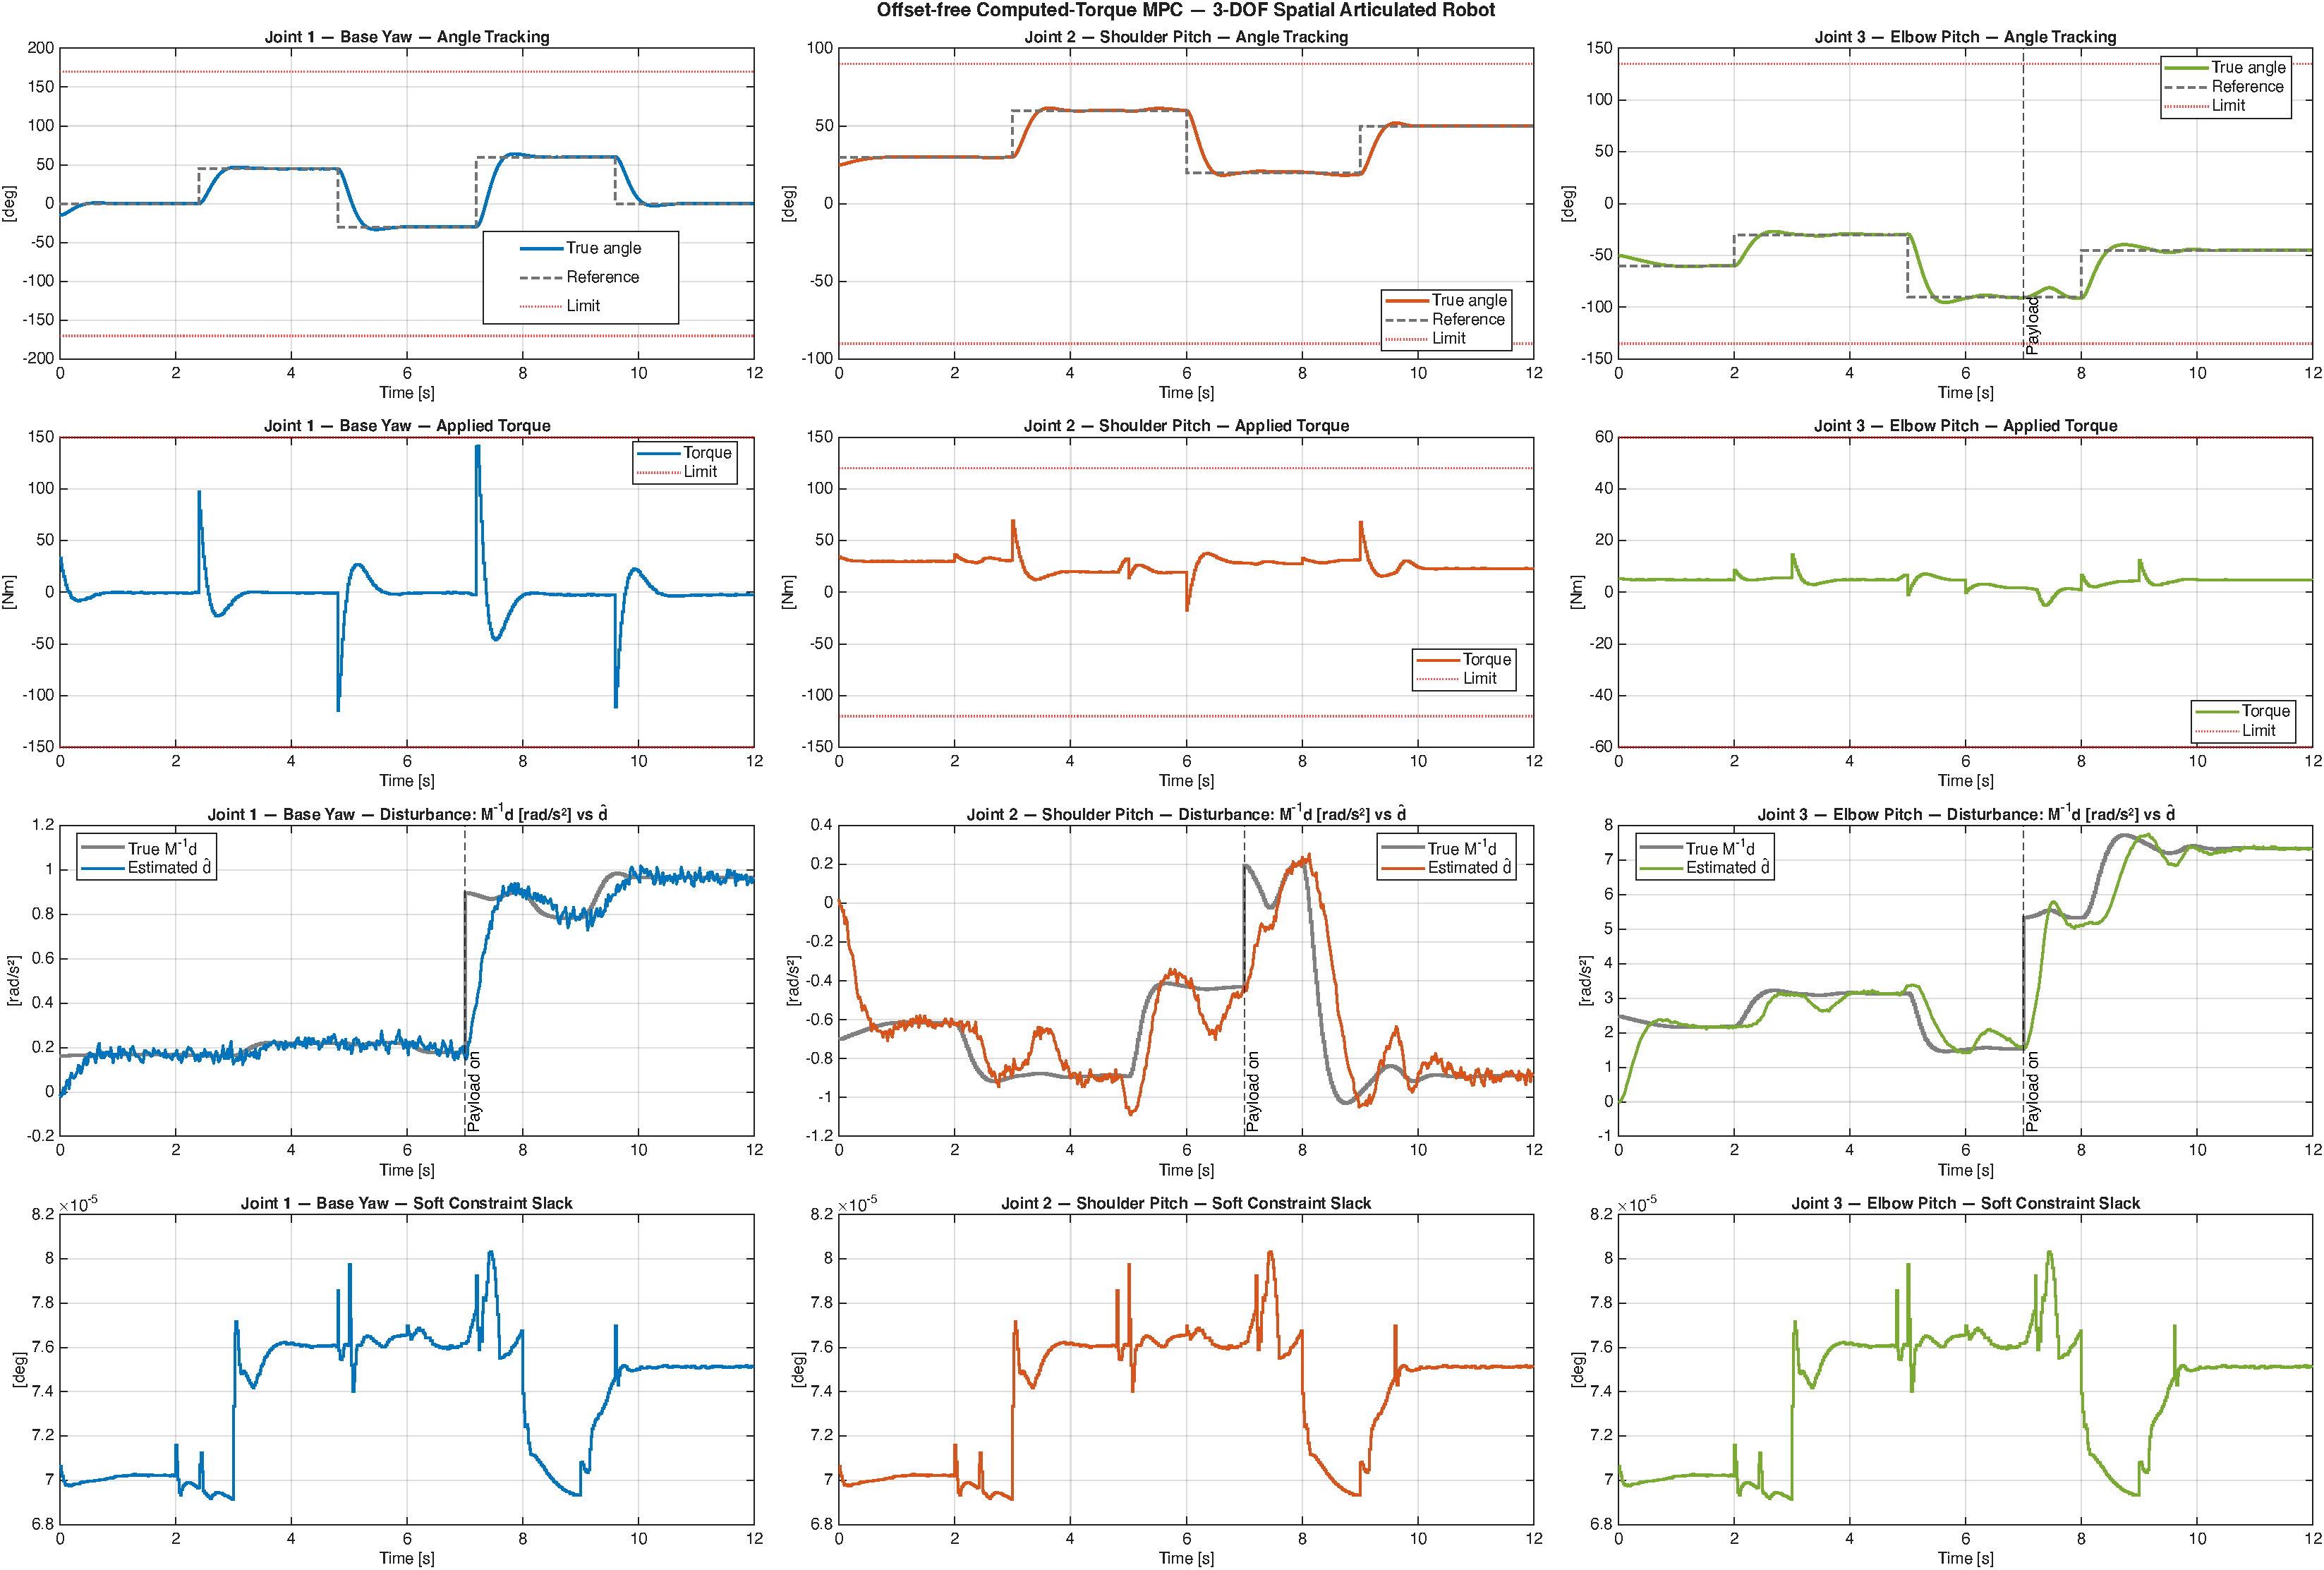
\includegraphics[width=1\linewidth]{Figures/Robot}
	    \captionof{figure}{Closed-loop performance of the offset-free computed-torque MPC applied to a 3-DOF spatial RRR articulated robot manipulator. The controller combines feedback linearisation (computed-torque law) with a deviation-form quadratic MPC ($N=15$, $T_s=20$\,ms) and an augmented Kalman filter for disturbance estimation. \textbf{Row~1}: Joint angle tracking for base yaw ($q_1$), shoulder pitch ($q_2$), and elbow pitch ($q_3$), with piecewise-constant reference trajectories (dashed) and joint limits (dotted red). \textbf{Row~2}: Applied actuator torques with saturation limits at $\pm150$, $\pm120$, and $\pm60$\,Nm, respectively. \textbf{Row~3}: Comparison of the true disturbance acceleration $M^{-1}(q)\,d$ (grey) and the Kalman filter estimate $\hat{d}$ (coloured), showing convergence after the payload step at $t=7$\,s. \textbf{Row~4}: Soft-constraint slack variables, which remain near zero throughout, confirming that joint limits are respected without significant violation. Constant friction biases ($0.5$, $-0.3$, $0.2$\,Nm) act on all joints from $t=0$, and an additional payload disturbance ($2.0$, $1.5$, $0.8$\,Nm) is applied at $t=7$\,s. The target calculator drives steady-state offsets to zero in all cases, demonstrating robust offset-free tracking despite unmodelled friction, sudden payload changes, and encoder noise ($\sigma=0.05^\circ$).}
	
		\label{fig:robot}


\end{examplebox}

\section*{Exercises}
\begin{enumerate}
	\item \textbf{Augmented State-Space Construction.}
	Consider a scalar plant
	\[
	x_{k+1} = 0.8\,x_k + u_k + d_k, \qquad y_k = x_k,
	\]
	where \(d_k\) is an unknown constant disturbance (\(d_{k+1}=d_k\)).
	\begin{enumerate}
		\item Define the augmented state vector \(z_k = [x_k,\; d_k]^T\) and write down the augmented system matrices \(A_{\mathrm{aug}}\), \(B_{\mathrm{aug}}\), and \(C_{\mathrm{aug}}\).
		\item Now suppose the disturbance enters only through the output, i.e.\ \(B_w = 0\) and \(C_d = 1\). How do the augmented matrices change?
		\item For the two-state system
		\[
		A = \begin{bmatrix} 1 & 0.1 \\ 0 & 0.95 \end{bmatrix}, \quad
		B = \begin{bmatrix} 0.005 \\ 0.1 \end{bmatrix}, \quad
		B_w = B, \quad
		C = \begin{bmatrix} 1 & 0 \end{bmatrix}, \quad C_d = 0,
		\]
		write out the full augmented matrices \(A_{\mathrm{aug}} \in \mathbb{R}^{3\times 3}\), \(B_{\mathrm{aug}} \in \mathbb{R}^{3\times 1}\), and \(C_{\mathrm{aug}} \in \mathbb{R}^{1\times 3}\).
	\end{enumerate}

	\item \textbf{Detectability of the Augmented System.}
	For the augmented pair \((A_{\mathrm{aug}},\, C_{\mathrm{aug}})\) constructed in Exercise~1(c):
	\begin{enumerate}
		\item Form the observability matrix
		\[
		\mathcal{O} = \begin{bmatrix} C_{\mathrm{aug}} \\ C_{\mathrm{aug}} A_{\mathrm{aug}} \\ C_{\mathrm{aug}} A_{\mathrm{aug}}^2 \end{bmatrix}
		\]
		and verify that its rank equals the dimension of the augmented state.
		\item Now suppose the system has two outputs \(y_k = C x_k\) with \(C = I_{2\times 2}\) and two independent disturbance states \(d_k \in \mathbb{R}^2\) with \(B_w = B\) and \(C_d = 0\). Does the augmented pair remain detectable? Justify your answer by examining the eigenvalues and the rank of the detectability test matrix \(\begin{bmatrix} A_{\mathrm{aug}} - \lambda I \\ C_{\mathrm{aug}} \end{bmatrix}\) at the eigenvalue \(\lambda = 1\).
		\item Explain the practical rule of thumb relating the number of disturbance states \(n_d\) to the number of measured outputs \(n_y\).
	\end{enumerate}

	\item \textbf{Steady-State Target Calculation.}
	Consider the system from Exercise~1(c) with the reference \(r_k = 2\) and a disturbance estimate \(\hat{d}_k = 0.5\).
	\begin{enumerate}
		\item Write out the target-calculator linear system
		\[
		\begin{bmatrix} I - A & -B \\ C & 0 \end{bmatrix}
		\begin{bmatrix} x_{ss} \\ u_{ss} \end{bmatrix}
		=
		\begin{bmatrix} B_w \hat{d}_k \\ r_k - C_d \hat{d}_k \end{bmatrix}
		\]
		with all numerical entries substituted.
		\item Solve for \(x_{ss}\) and \(u_{ss}\). Verify that the steady-state output satisfies \(C x_{ss} = r_k\).
		\item Suppose the input is constrained to \(-1 \le u \le 1\). Is the steady-state target \(u_{ss}\) feasible? If not, explain qualitatively how a constrained steady-state optimisation (as in Equation~\eqref{eq:target_qp}) would handle this situation.
	\end{enumerate}

	\item \textbf{Deviation-Form MPC Variables.}
	Using the targets \((x_{ss}, u_{ss})\) computed in Exercise~3:
	\begin{enumerate}
		\item Suppose the current state estimate is \(\hat{x}_k = [1.5,\; 0.3]^T\). Compute the initial deviation \(\tilde{x}_0 = \hat{x}_k - x_{ss}\).
		\item Write out the deviation-form prediction model \(\tilde{x}_{i+1} = A \tilde{x}_i + B \tilde{u}_i\) and explain why the disturbance estimate \(\hat{d}_k\) does not appear in this equation.
		\item If the hard input constraints are \(-1 \le u_k \le 1\), express these as constraints on the deviation input \(\tilde{u}_i\). Are the deviation-form constraints symmetric about zero?
		\item Explain the role of the terminal cost matrix \(P_{\mathrm{term}}\) in the MPC cost function~\eqref{eq:mpc_problem} and state how it is typically computed.
	\end{enumerate}

	\item \textbf{Effect of Misspecified \(B_w\).}
	Suppose the true plant has the disturbance entering through \(B_w^{\mathrm{true}} = [0;\; 1]\), but the augmented observer and target calculator are designed using the incorrect assumption \(B_w = B = [0.005;\; 0.1]\).
	\begin{enumerate}
		\item Will the augmented Kalman filter still converge to a constant disturbance estimate \(\hat{d}_k\) in steady state? Explain why or why not.
		\item At steady state, the target calculator enforces \((I-A)x_{ss} = B u_{ss} + B_w \hat{d}_k\) and \(C x_{ss} = r_k\). Does the controller still achieve zero steady-state output offset despite the mismatch in \(B_w\)? Argue from the structure of the equilibrium equations.
		\item Discuss the transient consequences of the misspecified \(B_w\). In particular, how might the transient response and the value of \(\hat{d}_k\) differ from the correctly specified case?
	\end{enumerate}

	\item \textbf{Comparison: MPC With and Without Disturbance Estimation.}
	Consider a standard (non-augmented) MPC regulator that uses the nominal model \(x_{k+1} = A x_k + B u_k\) without disturbance estimation, alongside the offset-free architecture of Algorithm~\ref{alg:offset_free_mpc}.
	\begin{enumerate}
		\item Suppose a constant disturbance \(d_k = d \neq 0\) acts on the plant through \(B_w\). Explain why the standard MPC regulator generally produces a non-zero steady-state tracking error. What is the source of the persistent offset?
		\item In the offset-free architecture, identify which component provides integral-action-like behaviour. How does the integrating disturbance model \(d_{k+1} = d_k\) relate to classical integral action?
		\item Suppose instead that the disturbance is sinusoidal, \(d_k = \sin(\omega k)\). Will the offset-free MPC with a constant disturbance model (\(d_{k+1} = d_k\)) eliminate the steady-state tracking error in this case? Justify your answer in terms of the internal model principle.
		\item Briefly outline how the disturbance model could be modified to handle the sinusoidal case.
	\end{enumerate}
\end{enumerate}
